\documentclass[12pt,a4paper]{report}
\usepackage[utf8]{inputenc}		% Pour afficher les caractères internationaux
%\usepackage{fourier}
\usepackage[T1]{fontenc}			% Pour l'encodage de caractères
\usepackage[french,english]{babel}


\usepackage{lmodern} % Pour changer le pack de police
\usepackage{makeidx} % For table of content
\usepackage{layout}  % For \Layout comment 

\usepackage{graphicx}   % For images 
\usepackage{subcaption} % for multiple image captions

\usepackage{rotating}


% ========= FOR LINKS IN TABLE OF CONTENT ============= % 
\usepackage{color}      % May be necessary if you want to color links
\usepackage{hyperref}   % clickable links 
\hypersetup{
    colorlinks=true,    %set true if you want colored links
    linktoc=all,        %set to all if you want both sections and subsections linked
    linkcolor=black,    %choose some color if you want links to stand out
}

\usepackage{float}      %used for figure placement with H as a parameter
\usepackage{setspace}
\usepackage{enumerate}  %like itemize but  with numbers %didnt use it yet
\usepackage{array}

% Bibliography 
% \usepackage[backend=bibtex,sorting=none]{biblatex}
% \addbibresource{bibliographie}

\usepackage[font=small,labelfont=bf]{caption}
\def\figurename{\textbf{Figure }}

%\PrerenderUnicode{é} % This is for fixing the issue or having index/header 'é' error

%------- stuff i did not use yet -----%
\usepackage{wrapfig} %pour que je mets la photo next to the text
\usepackage{fancyhdr}
%\usepackage{tabu}
%\usepackage[final]{pdfpages}        % To Include PDFs
%------------------------------------%



%\usepackage{fourier}
\title{Projet Fin Etude}
\author{Benzerga Malek}
\date{\today}

%------------ pour le title head ------------%



\usepackage{fancyhdr}
\pagestyle{fancy}
\fancyhf{}

\fancyhead[RE,LO]{\rightmark}
\fancyfoot[CE,CO]{\thepage}


%-------------------------------------------%

\providecommand{\keywordEN}[1]{\textbf{\textit{Keywords---}} #1}

\providecommand{\keywordFR}[1]{\textbf{\textit{Mots clés---}} #1}

\providecommand{\keywords}[1]{\textbf{\textit{Mots clés---}} #1}
\providecommand{\keywordz}[1]{\textbf{\textit{Keywords---}} #1}


\hypersetup{
pdftitle={Traitement,Analyse de Donnèes pour l'Evaluation de la Qualitè de la Route},
pdfsubject={Projet de Fin d’Etudes},
pdfauthor={Benzerga Malek},
pdfkeywords={Sensors, Animalies,Road, Accelerometre, Android, flutter}
}

\begin{document}



\selectlanguage{french} 
	\begin{abstract}

        L'importance des infrastructures routières pour la société pourrait être comparée à celle des vaisseaux sanguins pour l'homme. Pour assurer la qualité de la surface de la route, elle doit être surveillée en permanence et réparée si nécessaire, et c'est le cœur du concept de ce travail.

        Dans ce projet, trois points majeurs seront abordés : la détection mobile et les différents avantages qu’elle offre, comment nous pouvons les utiliser pour détecter les anomalies routières ( mentionnant plusieurs travaux similaires et présentant l’algorithme que nous avons utilisé pour fabriquer notre système), et enfin, présenter l’ensemble du système depuis l’application d’enregistrement pour mettre en place en passant par la partie serveur, et jusqu’aux résultats. \newline 




		\begin{keywords}
			Détection Mobile, Algorithmes, Anomalies, Seuil, Capteurs de smartphone, Accelerometres, Flutter.
		\end{keywords}
		

		
		
	\end{abstract}
	
	\begin{selectlanguage}{english}
		
		\begin{abstract}
            
            The importance of road infrastructure for society could be compared to that of blood vessels for humans. To ensure the quality of the road surface, it must be continuously monitored and repaired if necessary, and that is the heart of this work.

            In this project, three major points will be addressed: mobile detection and the various advantages it offers; how we can use them to detect road anomalies mentioning several similar works and presenting the algorithm that we used to build our system, then present the whole system from the recording application going through the server part to the results. \newline 

			\begin{keywordEN}
				Mobile Sensing, Algorithms, Anomalies, Threshold, Smartphone Sensors, Accelerometers, Flutter.\\
				
			\end{keywordEN}
			
		\end{abstract}
    \end{selectlanguage}
	
	
\tableofcontents
\listoffigures

\chapter*{Introduction générale}
\renewcommand{\thesection}{\arabic{section}}
		
 \addcontentsline{toc}{chapter}{Introduction générale}



\label{chapitre1}
		
		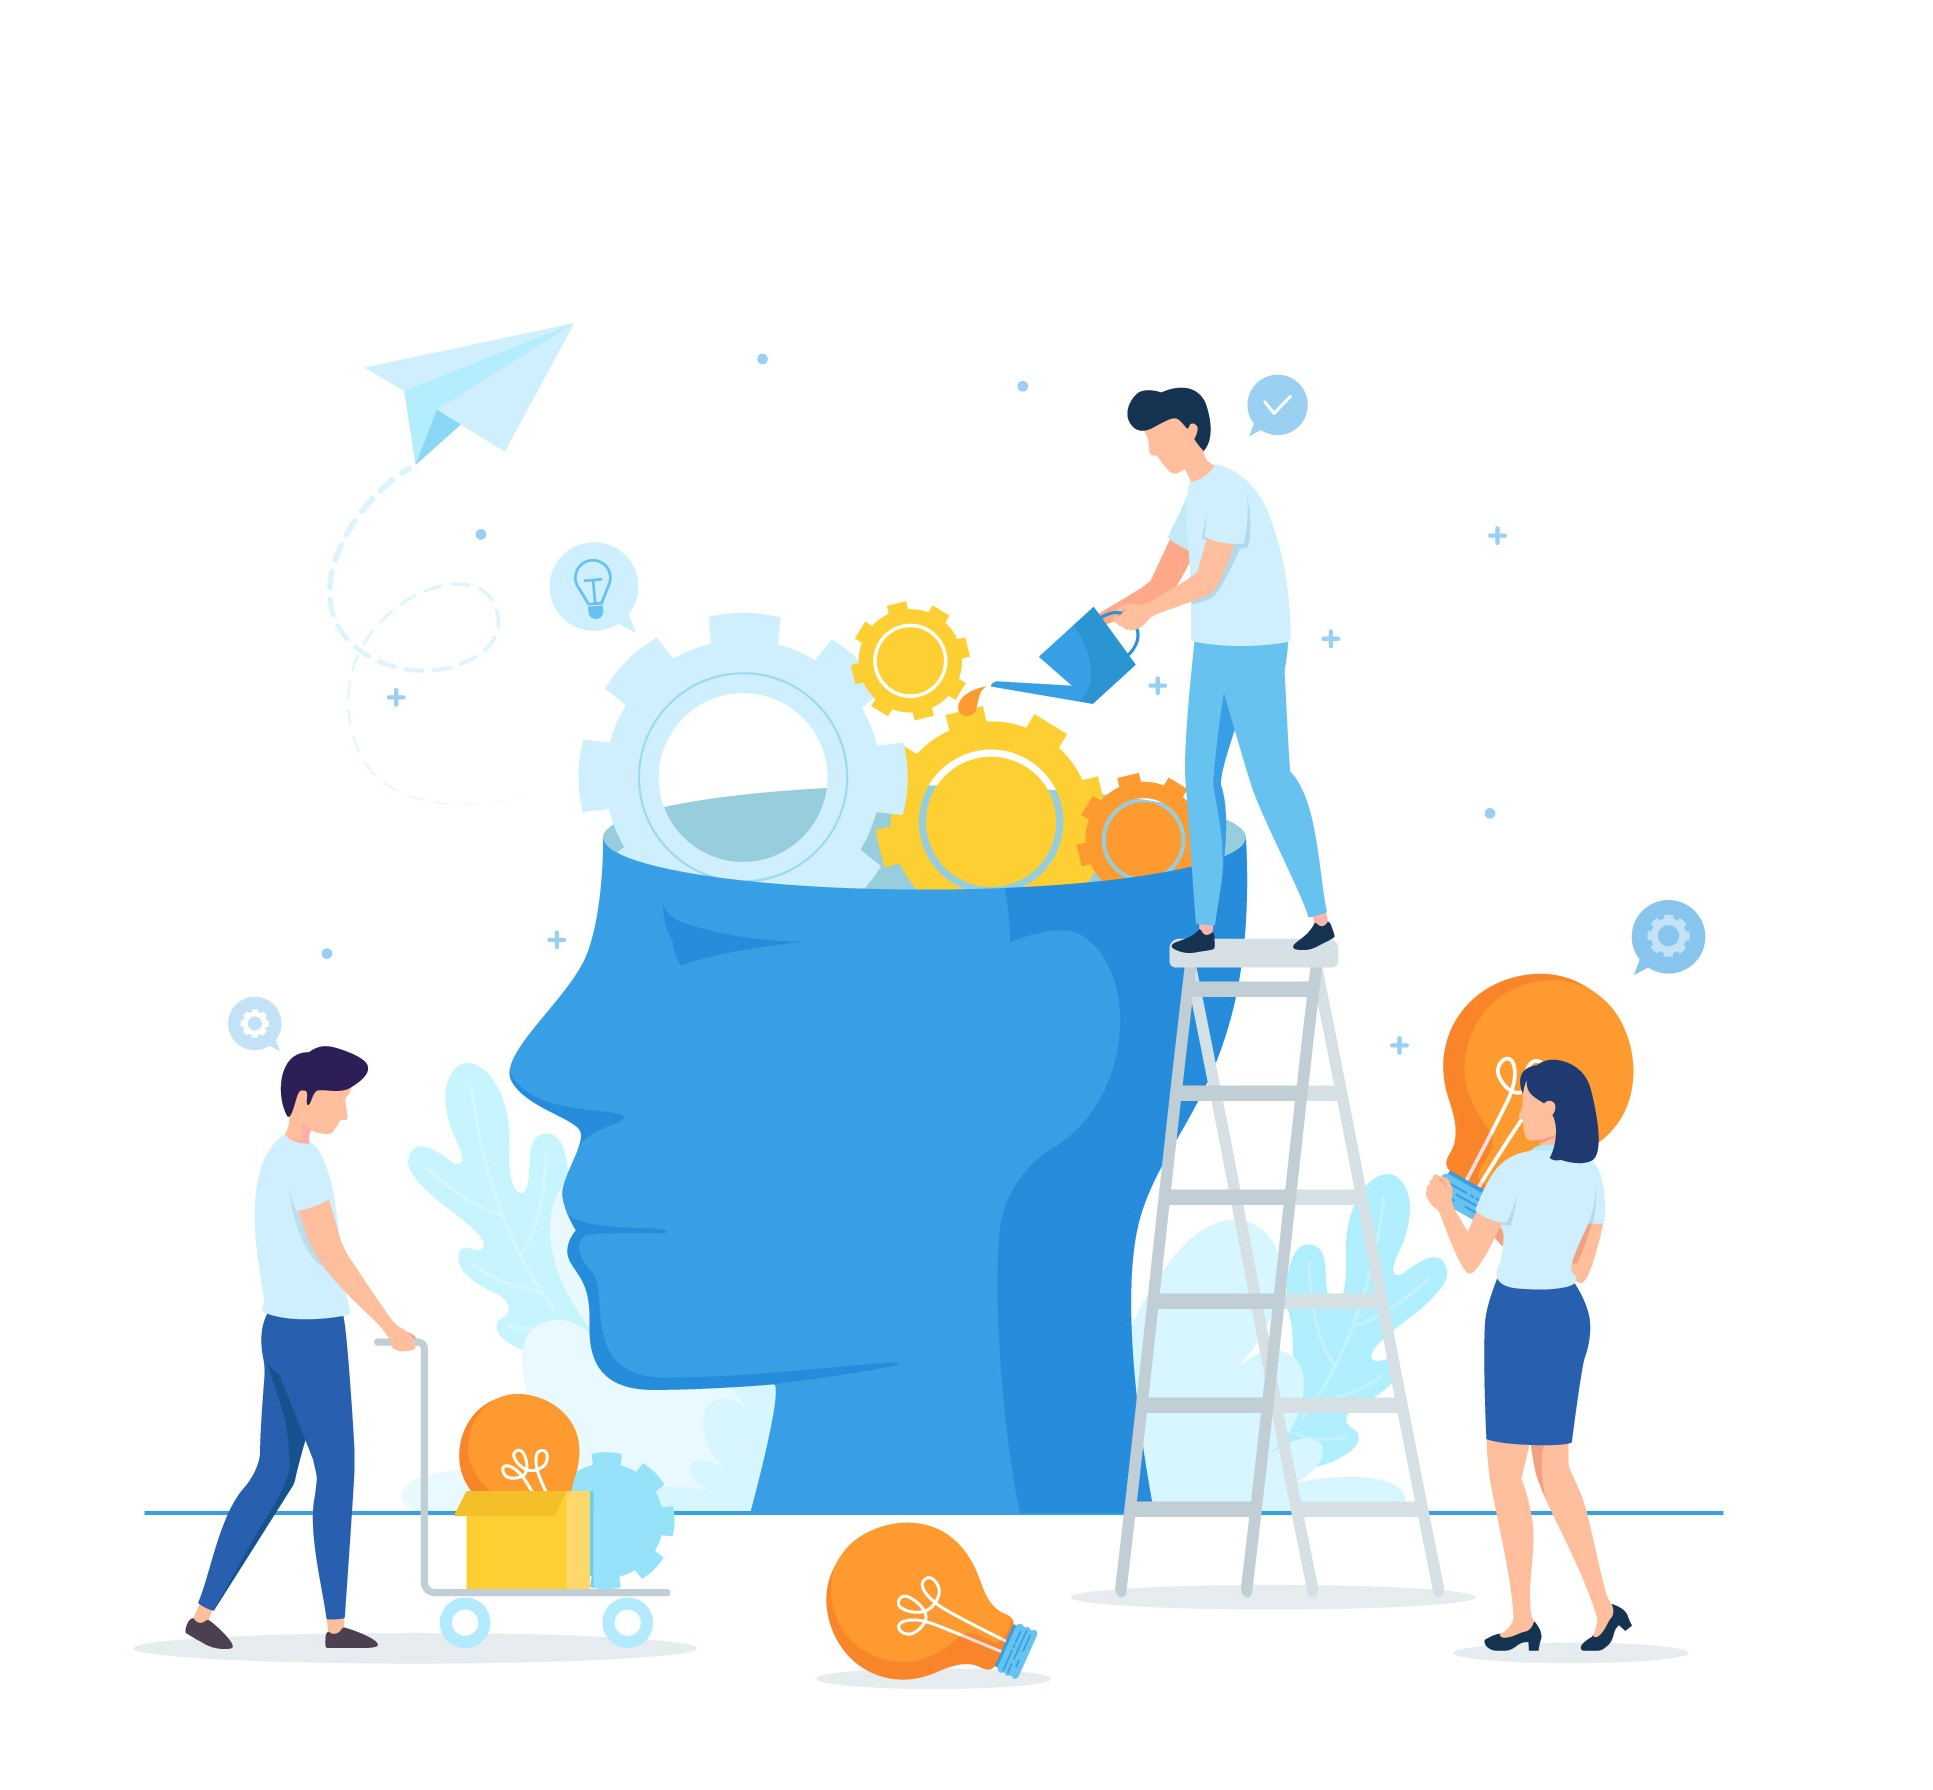
\includegraphics [width=1 \linewidth, height=0.8\textheight, keepaspectratio] {Images/chapterFigures/chOne.png}
		
	
		
    \newpage
    \thispagestyle{plain}
Selon le centre national de prévention et de sécurité routière algérien :
plus de 3.049 personnes avaient trouvé la mort et 29.095 personnes avaient été blessées
dans 21.109 accidents enregistrés au niveau national lors des onze premiers mois de l'année 2019  \cite{nassimaAccidentsRouteAlger}.
\begin{figure}[h!]
  \center
  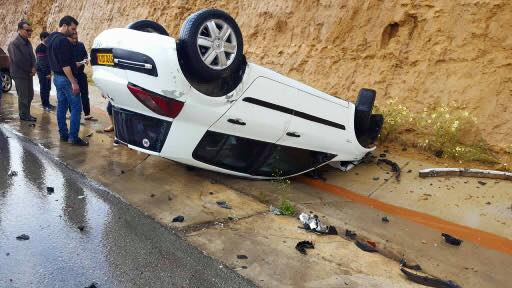
\includegraphics[width=0.75\textwidth]{Images/chapter1/accident.jpg}
  \caption{Accident de route.}
  \label{fig:Accident}
\end{figure}
Dans un scénario réel, la règle dit que plus la surface de la route est confrontée
à des changements de climat (entre le froid et le chaud) et avec un manque de soins,
plus elle subit des dégâts et affecte ensuite la vie des gens.

La surveillance de la surface des routes est un problème difficile dans le domaine des
infrastructures de transport routier dans le monde entier. Une zone en mauvais état peut
endommager les véhicules, les conducteurs et même provoquer un accident.
Au regard d'autre pays étrangés, ils sont également à l'origine de poursuites et de dommages-intérêts coûteux, par exemple,
en 2005, l'État du Michigan avait déposé plus de 7,500 réclamations pour dommages liés
aux nids-de-poule \footnote{http://www.detnews.com/2005/specialreport/0510/18/A01-350197.htm}, et les
compagnies d'assurance recevaient plus de 500,000 réclamations pour nids-de-poule chaque
année\footnote{http://www.wktv.com/special/6733696.html}.

Les municipalités du monde entier dépensent des millions de dollars pour entretenir et réparer leurs routes.
Malgré cet investissement, peu de gens sont satisfaits de la qualité de la route où ils vivent ou travaillent, car c'est  toujours trop tard!!

\section{Problématique}
De ce qui précède, l'entretien et la maintenance de la qualité de l'infrastructure routière est d'une importance vitale pour la société.

En Algérie, particulièrement, ce domaine est presque négligé, les routes endommagées sont plus nombreuses que les routes sûres.
L'entretien de la route en Algérie  passe par plusieurs phases :

\renewcommand{\labelitemi}{$\bullet$}
\begin{itemize}
  \item Détection des dégradations.
  \item Localisation des dégradations : les agents du service de contrôle de la route utilisent les points kilométriques 'PK'. pour localiser les dégradations.
  \item L'entretien de la route se fait soit par la Direction des Travaux Publics 'DTP' ou une entreprise désignée par le Ministère des Travaux Publics 'MTP'.
\end{itemize}

La détection des dégradations jusqu'à présent se fait par constatation visuelle par des agents d'entretien de la DTP, cette étape est fastidieuse et longue nécessitant un savoir-faire particulier et une expérience dans le domaine. Par conséquent les dégradations (nids-de-poule/bosses) prennent beaucoup de temps pour être réparées et par conséquent elles causeront plus de dégâts.

\section{Anomalies dans une route}
Dans nos recherches lors de l'étude de cette problématique, nous observons que les anomalies
les plus courantes sont les nids-de-poule (potholes) et les bosses (bumps).
Ces deux catégories peuvent classer la plupart des anomalies trouvées dans notre vie quotidienne.

\subsection{Les fissures}
La fissuration est une dégradation majeure qui touche l'ensemble des chaussées avec différentes origines et différents mécanismes de développement. Elle est à la source d'une accélération des dégradations propres à chaque type de chaussée par la diminution de la portance du support lors de l'infiltration d'eau et par la perte des conditions mécaniques nécessaires au maintien de la résistance des matériaux \cite{FissurationOrnierageProblematiques}.

\begin{figure}[h!]
  \center
  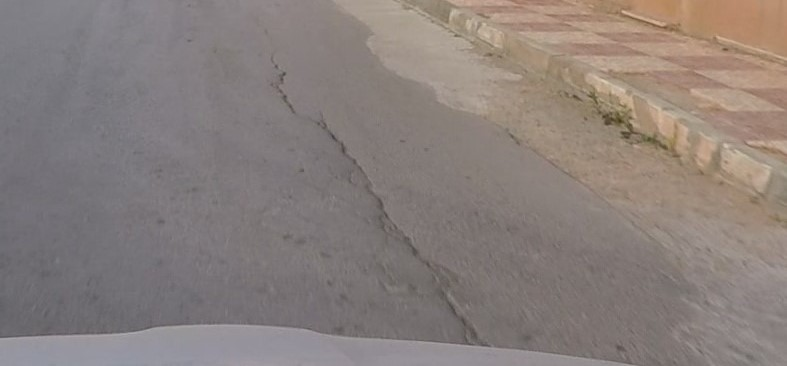
\includegraphics[width=0.75\textwidth]{Images/chapter1/fissures.jpg}
  \caption{Une fissure -Oran.}
  \label{fig:Technologies}
\end{figure}


\textbf{Causes probables :}
\renewcommand{\labelitemi}{$\bullet$}
\begin{itemize}

  \item Mauvaise construction du joint longitudinal entre deux bandes d'enrobés.
  \item Fatigue de la chaussée due à une structure insuffisante vis-à-vis du trafic
        ou une portance, du sol support insuffisante.
  \item Les caractéristiques du sol : tassement, retrait du sol argileux à la suite
        d'une longue période de sécheresse (Assèchement).
\end{itemize}


\subsection{les nids-de-poule}

Les nids-de-poule sont principalement causés par une mauvaise qualité de la chaussée ou des problèmes sous la surface.

\begin{figure}[h!]
  \center
  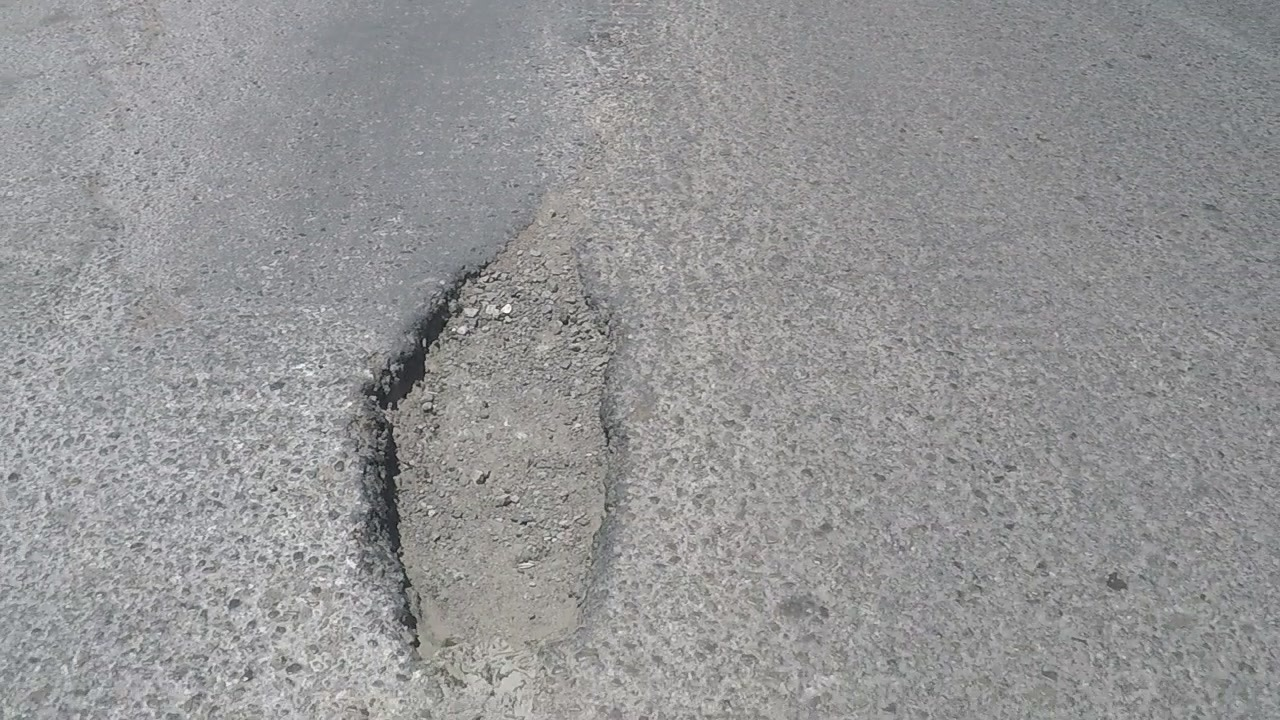
\includegraphics[width=0.75\textwidth]{Images/chapter1/Pothole.jpg}
  \caption{Nid-de-poule -Oran.}
\end{figure}

Un nid-de-poule est une dépression dans la surface d'une route, généralement une chaussée asphaltée, où la circulation
a enlevé des morceaux cassés de la chaussée.
C'est généralement le résultat de l'eau dans la structure du sol sous-jacente et du trafic passant sur la zone affectée.
L'eau affaiblit d'abord le sol sous-jacent; le trafic fatigue et brise la surface asphaltée mal supportée de la zone touchée.
L'action continue de la circulation éjecte l'asphalte et le sol sous-jacent pour créer un trou dans la chaussée.
\footnote{https://en.wikipedia.org/wiki/Pothole}



\subsection{Les Ralentisseurs (longs et courts)}

Normalement fabriquées par l'homme et généralement utilisées pour ralentir les véhicules à proximité des passages pour piétons.

On constate le plus souvent qu'ils imposent une limite de vitesse basse, inférieure à 40 km/h ou moins poussant les conducteurs à freiner d'avance.
Les ralentisseurs en général ne sont pas des anomalies, mais les ralentisseurs mal faits ou ceux qui ont été exposés à des dégâts sans réparation sont considérés comme des anomalies.
De plus, leur utilisation est parfois controversée car:

\begin{figure}[h!]
  \center
  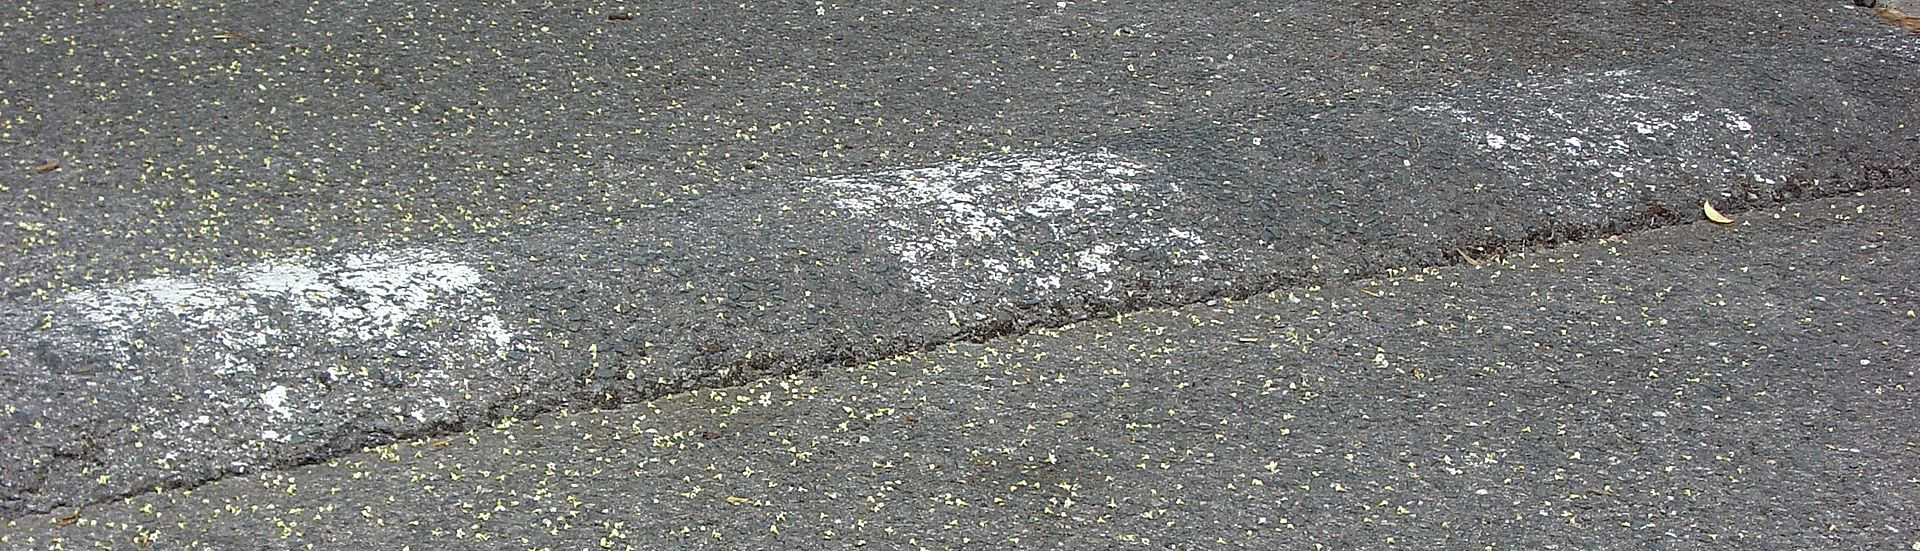
\includegraphics[width=0.75\textwidth]{Images/chapter1/Speedbump.jpg}
  \caption{Ralentisseurs -Mostaganem.}
\end{figure}
\renewcommand{\labelitemi}{$\bullet$}
\begin{itemize}
  \item Ils peuvent augmenter le bruit de la circulation.
  \item Peuvent endommager les véhicules s'ils sont traversés à une vitesse trop élevée et ralentir les véhicules d'urgence.
  \item Poussent le conducteur sur à freiner puis accélèrer, ce qui augmente considérablement la libération de gaz nocifs.
  \item Les ralentisseurs mal conçus qui se tiennent trop haut ou avec un angle
        trop aigu peuvent perturber les conducteurs et peuvent être difficiles à naviguer pour les véhicules à faible garde au sol,
        même à très basse vitesse. De nombreuses voitures de sport ont ce problème avec de tels ralentisseurs.
  \item Les ralentisseurs peuvent également présenter de graves dangers pour les motocyclistes et les cyclistes s'ils ne sont pas clairement visibles.
\end{itemize}

Les ralentisseurs coûtent entre 50 et 200 Dollar et peuvent devoir être remplacés au fil du temps
en raison de l'usure \cite{SpeedBump2020}.



\section{Objectifs et analyse des besoins}

Détecter les anomalies d'une route présente un vrai défi. Avant de commencer le projet,
nous sommes amenés à répondre aux questions suivantes :
\renewcommand{\labelitemi}{$\bullet$}
\begin{itemize}
  \item Quels sont les différents caractéristiques d'une anomalie?
  \item Quels sont les différentes difficultés et critères à prendre en compte pour décider si une anomalie est présente?
  \item Peut-on offrir une solution informatique évoluée pour assister à cette décision? Si oui :
        \begin{itemize}
          \item Comment mesurer le niveau de qualité d'une route?
          \item Comment détecter/révéler les différentes causes d'une mauvaise route?
          \item Comment localiser géographiquement chaque anomalie?
          \item Comment présenter cette solution aux services concernés de manière simple et efficace ?
        \end{itemize}
\end{itemize}

\section{Avantages}
Développer un outil de détection automatique de qualité de la route aurait pour apport:
\renewcommand{\labelitemi}{$\bullet$}
\begin{itemize}
  \item Un gain considérable de temps, efforts humains et une réduction de dépenses.
  \item Une surface de route solide et surtout sans danger pour les piétons et les conducteurs.
  \item Une meilleure circulation en ville en diminuant le nombre d'accidents de route et ainsi réduire les dégâts sur les véhicules.
\end{itemize}


\section{Solution proposée}
Nous proposons un outil permettant de :
\renewcommand{\labelitemi}{$\bullet$}
\begin{itemize}
  \item Fournir à la direction des travaux public "DTP" un moyen de se renseigner en temps réel sur la qualité des routes afin d'intervenir efficacement et le plus rapidement possible dans les travaux d'entretien. Ceci permettra d'améliorer les manques cités plus haut.
  \item Mieux assister le conducteur dans sa conduite en l'alertant  sur la qualité de la route, afin qu'il adapte sa conduite en fonction.
\end{itemize}

Pour cela, nous visons à développer un système qui proposera les fonctionnalités suivantes :
\renewcommand{\labelitemi}{$\bullet$}
\begin{itemize}
  \item Détecter les événements (les nids-de-poule et les ralentisseurs dans notre cas) en temps réel. La collecte de données brutes pour un post-traitement hors ligne.
  \item Utiliser un smartphone basé sur Android-OS avec des capteurs accéléromètres comme plate-forme matérielle / logicielle.
  \item Pouvoir fonctionner sur différents modèles de smartphones avec différents paramètres. Au cours du processus de mise en œuvre du système, l'ensemble des paramètres minimaux du smartphone doit être déterminé et décrit.
  \item Détecter les événements lors de la conduite dans différents types de véhicules à quatre roues tels que des voitures particulières, des mini-fourgonnettes et des bus. Les véhicules à deux roues tels que les motos et les scooters ne sont pas pris en compte.
\end{itemize}


\renewcommand{\thesection}{\thechapter.\arabic{section}}
















\chapter{La détection mobile}

\label{chapitre2}
		
		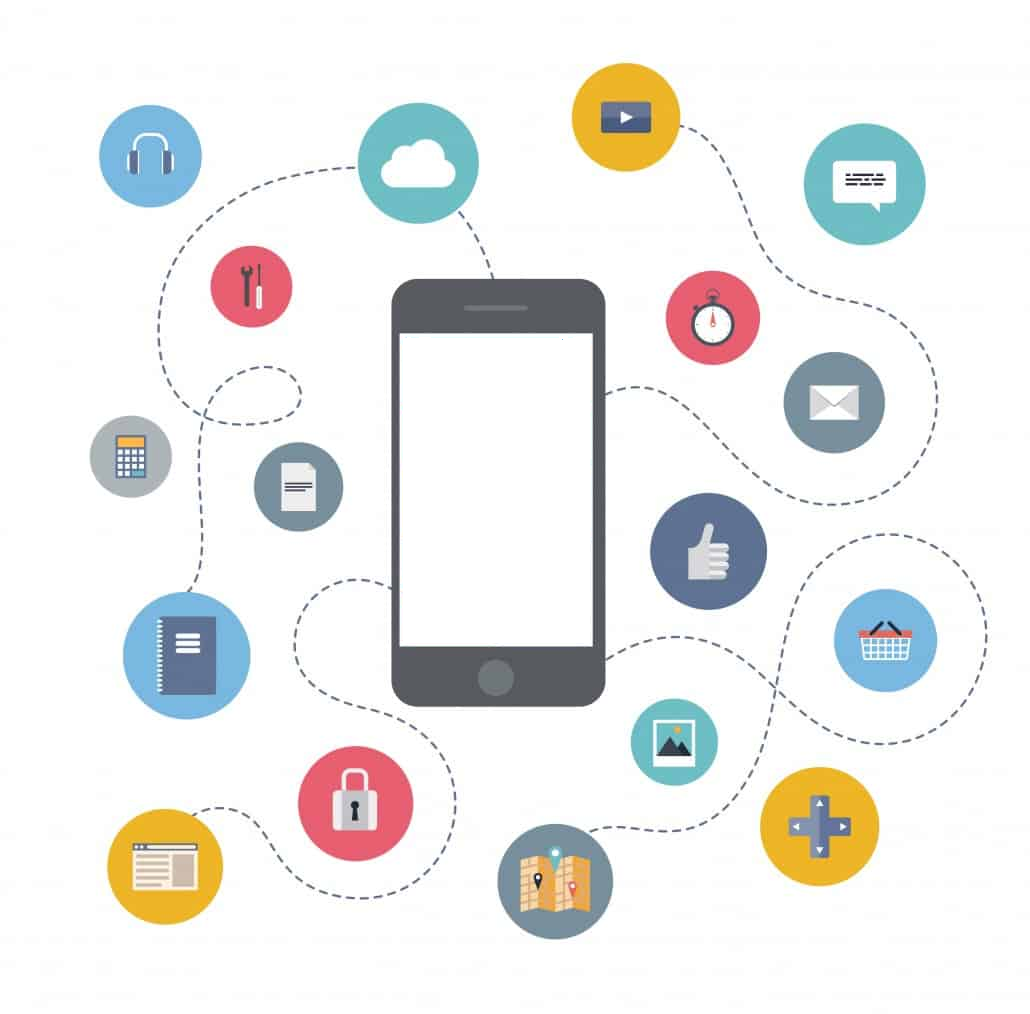
\includegraphics [width=1 \linewidth, height=0.8\textheight, keepaspectratio] {Images/chapterFigures/chTwo.png}
		
	
		
		\newpage

Récemment, des petits capteurs de haute performance se sont répandus et sont intégrés dans divers types d'objets dans notre environnement.

La détection mobile "Mobile sensing" utilise des capteurs intégrés dans des objets en mouvement tels que des voitures, des vélos et des smartphones, puis les considère comme des capteurs de détection \cite{nomuraMethodEstimatingRoad2015}.

De plus, le taux de propagation des smartphones de haute qualité augmente et continuera de le faire. Ces derniers incluent de différents types de capteurs tels que des capteurs d'accélération et des capteurs gyroscopiques.

%---- talking about sensors---%


\section{Différents Capteurs}

Le capteur est un appareil qui détecte les changements dans l'environnement proche et envoie ces données au système d'exploitation ou au processeur. Ils détectent et collectent les données pour lesquelles ils sont faits.

Il existe trois catégories principales de capteurs que possède un smartphone \cite{tilluMobileSensorsComponents2019}:

{\bf Les capteurs de mouvements:}
ils mesurent les forces d'accélération et les rotations autour des trois axes.  Ces capteurs sont capables de déterminer dans quelle direction est orienté l’appareil. A titre d’exemple, On trouve l'accéléromètre et le gyroscope.

    {\bf Les capteurs de position et d’attitude:}
Ce genre de capteurs détermine la position et l’orientation de l'appareil. On trouve donc les capteurs d’orientation, le gyroscope et le magnétomètre ainsi que le GPS.

    {\bf Les capteurs environnementaux:}
c’est des capteurs qui mesurent la pression atmosphérique, l'illumination et la température ambiante (Baromètre, photomètre et thermomètre).

\section{Capteurs d'un smartphone}

\subsection{Accéléromètre}
L'accéléromètre détecte les changements d'orientation des smartphones par rapport aux 3 axes orthogonaux (X, Y et Z). Cette accélération est utilisée pour déterminer la vitesse de l’appareil.

\begin{figure}[h!]
    \center
    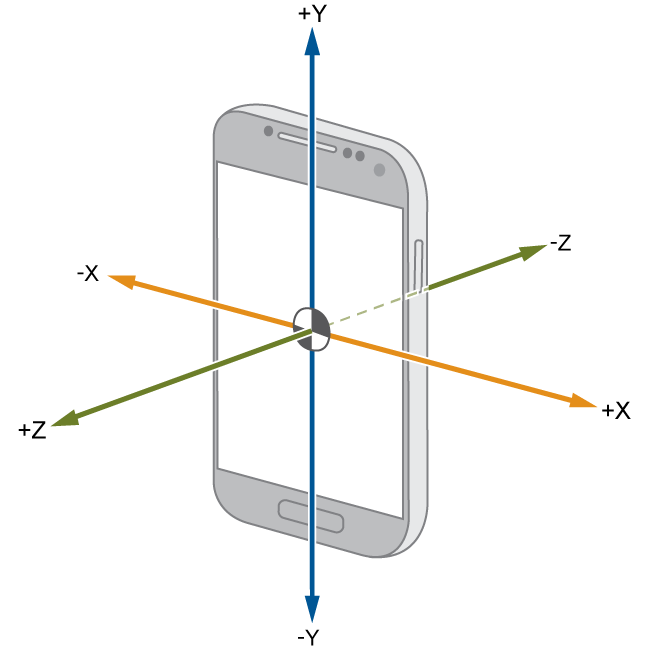
\includegraphics[width=0.60\textwidth]{Images/chapter1/axes.png}
    \caption{Axes orthogonaux utilisés}
    \label{fig:axis}
\end{figure}

\subsection{Gyroscope}
Le gyroscope ou capteur gyroscopique est une version avancée de l'accéléromètre. Alors que l'accéléromètre détecte la détection de mouvement basée sur l'axe, le gyroscope fonctionne avec l'accéléromètre et détecte chaque degré de changement d'orientation. Il fournit une détection de mouvement très précise.

\subsection{GPS}
Le GPS ou le système de positionnement global est également très courant dans la plupart des téléphones modernes. Il aide à localiser l'emplacement sur Terre et aide à la navigation.

\section{Applications utilisant la détection mobile.}
Avec l'évolution des smartphones, le monde a commencé à tirer de plus en plus d'avantages de leurs capacités pour développer de nombreuses applications mobiles. Dont certaines faisant usage des capteurs du smartphone pour réaliser et automatiser des tâches qui étaient avant impossibles sans des appareils sophistiqués.
\subsection{Galaxy Watch}
Galaxy Watch est une montre intelligente développée par Samsung Electronics. Elle embarque une multitude de capteurs : Accéléromètre, baromètre, capteur gyroscopique, capteur cardiaque électrique (ECG), capteur de fréquence cardiaque optique et un capteur de lumière.

Le capteur de fréquence cardiaque mesure votre fréquence cardiaque en battements par minute à l'aide d'une source de lumière LED optique et d'un capteur de lumière LED. La lumière brille à travers votre peau et le capteur mesure la quantité de lumière réfléchie. Les reflets de la lumière varient au fur et à mesure que le sang pulsera sous votre peau au-delà de la lumière.
\begin{figure}[h!]
    \center
    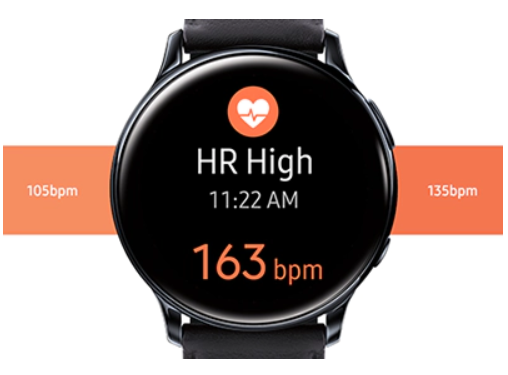
\includegraphics[width=0.5\textwidth]{Images/chapter1/galaxyWatch.PNG}
    \caption{Galaxy Watch}
    \label{fig:Application}
\end{figure}
\subsection{Uber}
Uber est un service de voiture à la demande qui vous permet de demander les services d'un chauffeur privé grâce à une application fonctionnant sur iPhone et Android. Ce service utilise un logiciel qui permet d'envoyer au chauffeur le plus proche votre localisation.

La cartographie est un élément clé du service de VTC (Voiture de transport avec chauffeur). Les opérateurs locaux d'Uber doivent en effet pouvoir visualiser en temps réel les chauffeurs qui circulent dans leur ville sans avoir à passer par des requêtes SQL fastidieuses.

Reposant sur le principe du géocodage inversé, la géolocalisation de l'adresse du points de prélèvement (position du client) est calculée par Uber en se basant sur la position GPS du smartphone du client. Côté VTC, un moteur de prédiction (basé sur des technologies de machine learning) oriente le chauffeur vers une destination plutôt qu'une autre en fonction notamment d'un historique clients. Enfin, Uber utilise aussi le suivi par GPS pour détecter les comportements dangereux au volant (notamment les excès de vitesse) et améliorer ainsi la sécurité routière.

\begin{figure}[h!]
    \center
    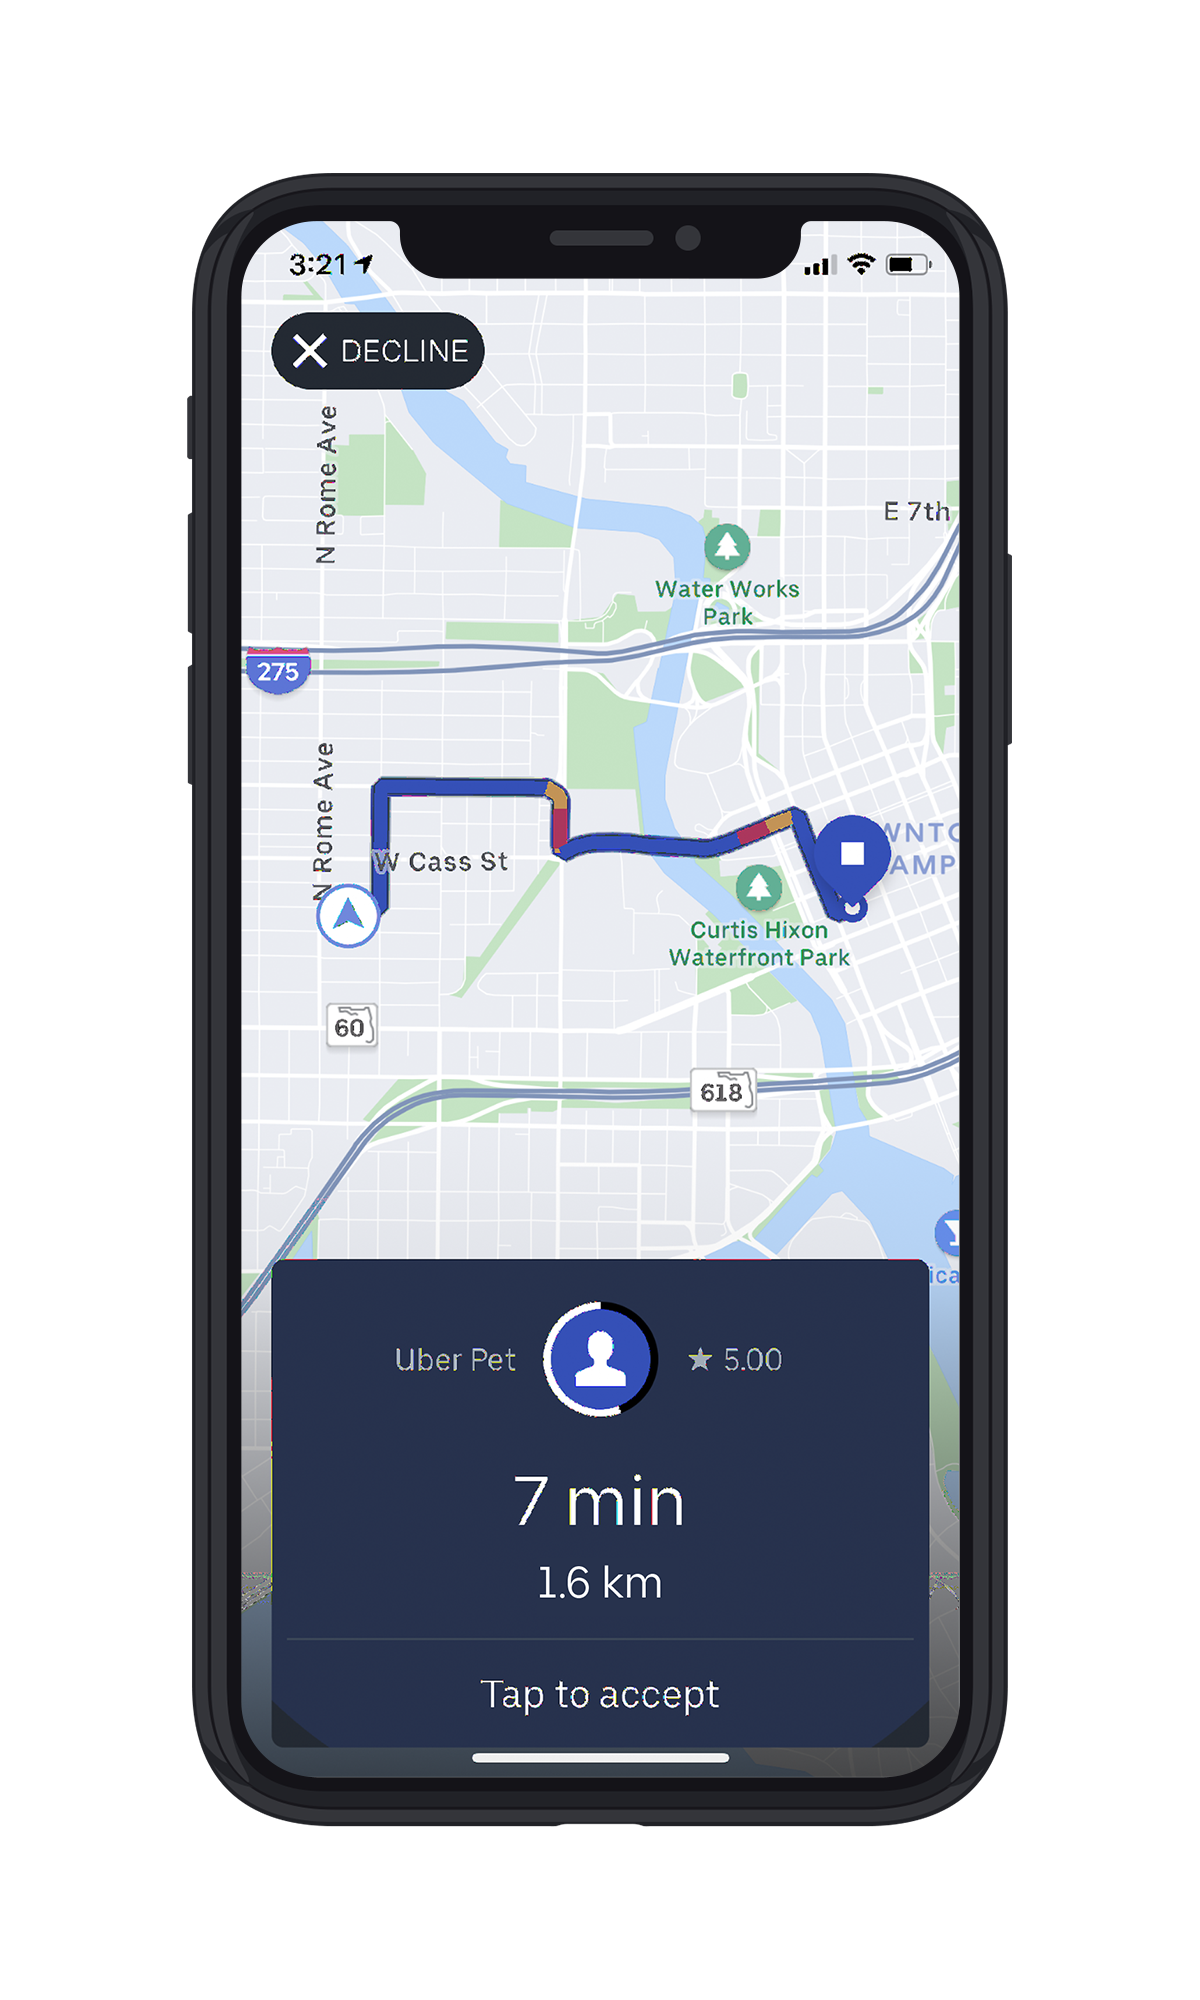
\includegraphics[width=0.4\textwidth]{Images/chapter1/uber.PNG}
    \caption{Uber}
    \label{fig:Application}
\end{figure}

\subsection{Samsung Health}
Samsung Health, à l'origine S Health, est une application gratuite développée par Samsung qui sert à suivre différents aspects de la vie quotidienne comme l'activité physique, l'alimentation et le sommeil.

Certaines fonctionnalités sont suivies par les entrées de l'utilisateur (nourriture / calories, poids, quantité d'eau, etc ...), et d'autres fonctionnalités sont suivies par des tests avec des accessoires de téléphone (Fitbit, Galaxy Active, Galaxy Fit, etc.) ou avec des capteurs de téléphone L'accéléromètre par exemple mesure l'accélération  dans de nombreux cas, par exemple: quand l'utilisateur fait du sport ou conduit sa voiture…

\textbf{Comment l'application mesure-t-elle les pas?}
Le smartphone détecte en permanence les mouvements du corps sur un accéléromètre à 3 axes. Les données sont enregistrées tout le temps qu'elles sont portées et allumées, ce qui permet au traqueur de suivre si l'individu marche en avant, court vite ou même immobile.

Les données collectées sont exécutées via un algorithme personnalisé. Cela permet au logiciel de détecter ce qu'impliquent réellement les différents mouvements enregistrés.

L'application permet à l'individu de savoir combien de pas ont été faits, à quelle vitesse, le rythme de l'individu, et même le nombre de calories susceptibles d'avoir été brulées. L'application permet à l'individu d'interagir avec les informations d'une manière conviviale.

\begin{figure}[h!]
    \center
    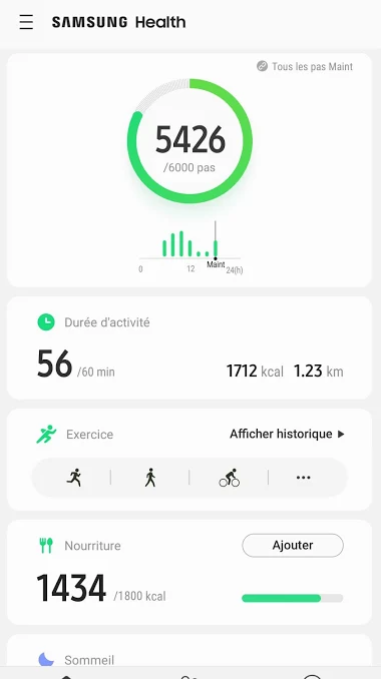
\includegraphics[width=0.33\textwidth]{Images/chapter1/samsungHealth.png}
    \caption{Samsung Health}
    \label{fig:Application}
\end{figure}


\chapter{Détection des anomalies de la route}

Avec cette évolution dans le domaine des mobiles, il est possible de développer un système pratique et efficace à faible coût et
 recueilli divers types d'informations afin de détecter la qualité de la surface des routes et aussi les anomalies routières telles
  que les ralentisseurs et les nids de-poule.

\section{Travaux Connexes}

\subsection{Wolverine}
Wolverine est \cite{bhoraskarWolverineTrafficRoad2012}une méthode non intrusive qui utilise  des données de capteurs des smartphones pour déterminer les conditions et l'état de la route, et utilise aussi des techniques d'apprentissage automatique “Machine learning” (clustering K-means et Support Vector Machine (SVM)) afin de la surveillance et suivi de l'état de la route
le chemin de ce travail consiste a deux étape: un algorithme pour réorienter virtuellement les axes de coordonnées d'un téléphone désorienté  et techniques d'apprentissage automatique pour identifier les événements de bosse et de freinage.\newline
Pour la 1ere étape ils ont développé une application qui traite les lectures de l'accéléromètre et du magnétomètre ainsi que les informations GPS et produit l'accélération linéaire du mobile, dans le cadre de référence du véhicule, ils ont développé un algorithme qui etude les axe x,y,z du téléphone et étude aussi les axes x’ y’ z’ de la véhicule.\newline
 La 2ème étape consistera à utiliser un algorithme d'apprentissage non supervisé de clustering K-means, avec K = 2, pour partitionner l'ensemble des points de données en deux classes; Ces classes sont ensuite étiquetées manuellement comme bosselées ou lisses (Bumby; smoothy)\newline
Une fois cet étiquetage manuel terminé, ils auront  un ensemble de points de données étiquetés. Ceux-ci sont ensuite utilisés pour former un classificateur Support Vector Machine. Ce SVM entraîné, à son tour, est utilisé pour classer les points de données qui sont générés pendant la phase de test, et donc pour prédire l'état du véhicule (Figure 2.1). \newline
\begin{figure}[h!]
  \center
  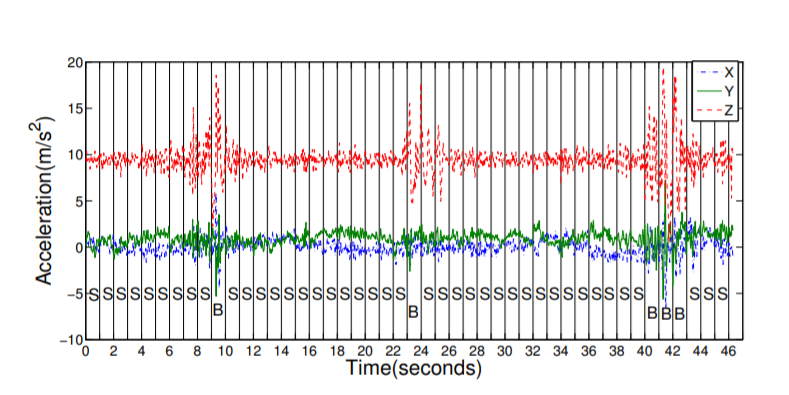
\includegraphics[width=0.75\textwidth]{Images/chapter2/relatedWork1.PNG}
 \caption{Accelerometer Data for three speedbreakers}
 \label{fig:graph}
  \end{figure}
  Et pour la détection du freinage du véhicule La technique utilisée est identique à celle de la détection des bosses,avec deux classes aussi étiquetées doux et freinage (smooth ‘S’, braking ‘R’) (Figure 2.2) :\newline
  \begin{figure}[h!]
    \center
    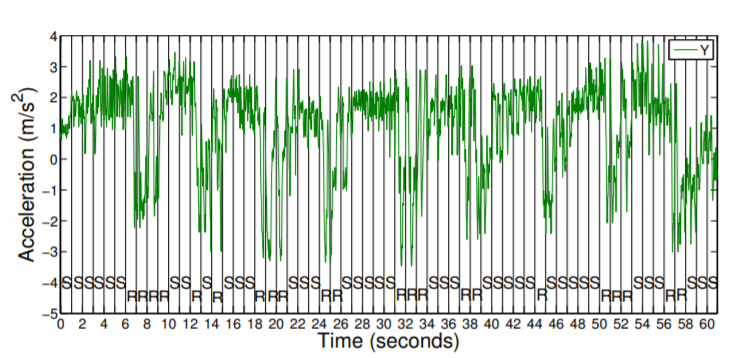
\includegraphics[width=0.75\textwidth]{Images/chapter2/relatedWork2.PNG}
   \caption{Braking events with generated class labels}
   \label{fig:graph}
    \end{figure}
    Ce  travail a été fait à Mumbai, L'algorithme identifie correctement 18 des 20 événements de bosse, Aucun tronçon de route lisse n'est identifié à tort comme une bosse. Ainsi, ils obtiennent un taux de faux négatifs de 10\% pour la détection des bosses et un taux de faux négatifs de 21,6\% et un taux de faux positifs de 2,7\% pour la détection de freinage.

  \subsection{Real time pothole detection using Android smartphones with accelerometer}
  Mednis et al., ont proposé un système de détection des nids-de-poule en temps réel basés sur des données d'accéléromètre pour le déploiement sur des appareils avec des ressources matérielles / logicielles limitées et leur évaluation sur des données du monde réel acquises à l'aide de différents téléphones intelligents basés sur Androïd OS. \newline
  ils ont utilisé un dispositif de collier LynxNet modifié \cite{PDFLynxNetWild} sur un route avec divers nids-de-poule pour la collecte des données des capteurs de l'accéléromètre.\newline 
  Après l'acquisition du premier data set de test, une recherche de fonctionnalités liées aux événements potentiels a été effectuée:\newline
  Le premier et le plus simple algorithme de détection d'événements ZTHRESH ont été testés sur l'ensemble de données acquis. Il est similaire à l'algorithme z-peak utilisé dans les systèmes Pothole Patrol \cite{PotholePatrolProceedings},Nericell\cite{mohanNericellUsingMobile2008}, et limite l'amplitude de l'accélération sur l'axe Z. Les caractéristiques qui classifient les mesures sont les valeurs dépassant des seuils spécifiques qui identifient le type des nids-de-pouls. \newline
  Pour la réorientation virtuelle, ils ont utilisé une approche plus simple: un placement contrôlé de l'accéléromètre, éliminant le traitement supplémentaire (Figure 2.3).\newline
  \begin{figure}[h!]
    \center
    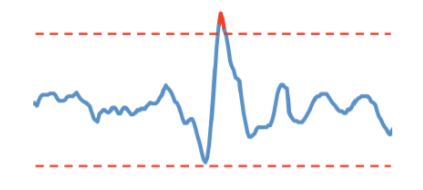
\includegraphics[width=0.75\textwidth]{Images/chapter2/relatedWork3.PNG}
   \caption{Pothole detection algorithm Z-THRESH. Events are represented by
   measurements with values exceeding specified threshold levels}
   \label{fig:graph}
    \end{figure}
    Ensuite, un algorithme légèrement plus avancé était le Z-DIFF (Figure 2.4) testé sur l'ensemble de données acquis. Contrairement à Z-THRESH, une recherche de deux mesures consécutives avec une différence entre les valeurs au-dessus du niveau de seuil spécifique a été effectuée. Ainsi, l'algorithme a détecté des changements rapides dans les données d'accélération verticale. L'algorithme nécessite la détermination de la position de l'axe Z de manière similaire à l'approche précédente. \newline
    \begin{figure}[h!]
      \center
      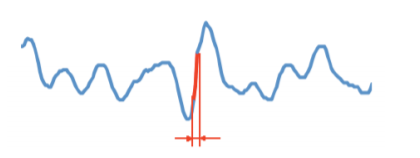
\includegraphics[width=0.75\textwidth]{Images/chapter2/relatedWork4.PNG}
     \caption{Pothole detection algorithm Z-DIFF. Events are represented by
     consecutive measurements with difference value above specific threshold level.}
     \label{fig:graph}
      \end{figure}
      les auteurs ont décidé de mettre en œuvre certaines des techniques utilisées pour le post-traitement. Une technique prometteuse pour la mise en œuvre sur un appareil à ressources limitées utilisait un écart type de l'accélération de l'axe vertical. Il a été implémenté dans l'algorithme STDEV (Z) (Figure 2.5) \newline

   \begin{figure}[h!]
      \center
      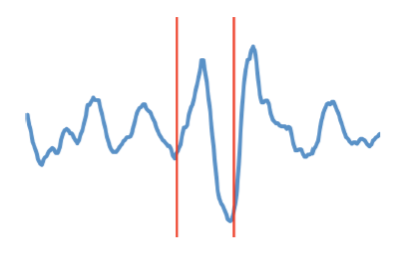
\includegraphics[width=0.75\textwidth]{Images/chapter2/relatedWork5.PNG}
     \caption{Pothole detection algorithm STDEV(Z). Events are represented by
     measurements with standard deviation value above specific threshold level.}
     \label{fig:graph}
      \end{figure}

      En utilisant des outils d'analyse visuelle de données et en recherchant des modèles de données spécifiques, les auteurs ont constaté qu'il existait certains événements caractérisés par un tuple de mesure spécifique. Toutes les données à trois axes de ce tuple avaient des valeurs proches de 0g. ils ont donc nommé cet algorithme G-ZERO (Figure 2.6).\newline


   \begin{figure}[h!]
      \center
      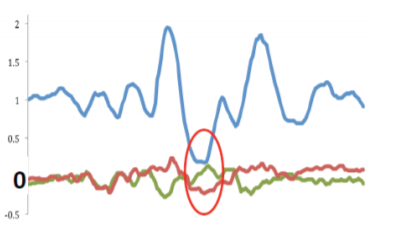
\includegraphics[width=0.75\textwidth]{Images/chapter2/relatedWork6.PNG}
     \caption{Pothole detection algorithm G-ZERO. Events are represented by tuple
     of measurements with all three axis values below specific threshold level.}
     \label{fig:graph}
      \end{figure}

      
les algorithmes ont détecté des irrégularités sur la route principale pour 100\% des grands nids-de-poule et 83 à 90\% des grappes de nids-de-poule; Selon l'algorithme, 78 à 89\% de la vérité terrain pour les petits nids-de-poule ont été détectés. Il est à noter que 9 d'entre eux (50\%) ont été détectés par les 4 algorithmes pour chacune des 10 sessions d'essai sur route
Et en gros, les tests d'évaluation ont abouti à une configuration optimale pour chaque algorithme sélectionné et l'analyse des performances dans le contexte de différentes classes d'irrégularité routière montre des taux de vrais positifs pouvant atteindre 90\%. \newline 



   Notre algorithme pour la détection de l'état de la route se distingue des travaux connexes de plusieurs côtés: \newline
Premièrement, nous ne détectons pas d'anomalies spécifiques, par contre nous concluons à l'état de la route en général. \newline
Deuxièmement, notre solution est plus simple en utilisant des ressources matérielles et logicielles limitées. \newline

\begin{table}[]
  \centering
  \resizebox{\textwidth}{!}{ %
  \begin{tabular}{lll}
    \hline
    Parameters & Wolverine & Mednis \\
    \hline
    Capteurs  & Accelerometre, Magnetometre, GPS  & Accelerometre, GPS \\
    \hline
Methodse pour la reorientation & Reorientation utilisant magnetometre et GPS bearing & Non défini \\
\hline
Valeur / Axes pris en compte & Z-axis Stdev sur une fenêtre de 1 sec du l'accéléromètre & Valeurs de l'axe Z de l'accéléromètre \\
\hline
Techniques utilisées & Machine Learning utilisé pour détecter les bosses et le freinage & Z-Thresh, ZDiff, STDEV, G-Zero \\
\hline
Taux d'échantillonnage réel de l'accéléromètre & 50 & 100 \\
\hline
Lieu d'expérimentation & IIT Bombay Campus & Vairoga iela, Riga, Latvia \\
\hline
Taux d'échantillonnage pris en compte par seconde & 50 values  & 100 values \\ 
\hline
Équipement utilisé pour la collecte de données & Capteurs de smartphone (Google Nexus S, HTC Wildfire S) & Samsung i5700 Samsung Galaxy S HTC Desire HTC HD2 \\
\hline
Véhicules utilisés & Suzuki Access 125, Autorickshaw & BMW 323 Touring (4-Wheeler) \\
\hline
Distance parcourue (km) / temps de trajet (heures) & Non reporté & 174 KM / Quelques semaines \\
\hline
Points de montage & Non défini (placé dans une certaine orientation arbitraire) & Tableau de bord avant \\
\hline
Objectif de la détection & Bosses, freinage & Nids de poule \\
\hline
Seuil 'threshold' utilisé & Non reporté & Z-Thresh = 0.4g Z-Diff = 0.2g STDEV = 0.2g G-Zero = 0.8g\\
\hline
Output & FN - 10\% (2 roues) FP - 8\% (3 roues) & 90\% des vrais positifs \\
\hline
Consommation d'énergie & Consomme 58\% moins d'énergie que Nericel & Non reporté \\
\hline
  \end{tabular} %
  }
  \caption{Inférences tirées Comparaison technique des travaux existants}
  \label{tab: my-table}
  \end{table}

  
  \section{L'acquisition des données}
  Notre système dépend de l'accéléromètre du smartphone attaché à un véhicule, produisant des résultats pour une condition de route donnée et sur la localisation précise de ces résultats à partir du GPS de ce smartphone.
Dans cette section, nous décrivons quelques expériences effectués par Pothole Patrol \cite{PDFPotholePatrol} pour valider le fonctionnement des capteurs d'un smartphone et la meilleure position où l'attacher.
\subsection{positionnement du smartphone}
Une préoccupation est que le placement du smartphone à l'intérieur du véhicule pourrait affecter la qualité du signal du capteur de l'accéléromètre. Pothole Patrol ont placé leurs accéléromètres à deux endroits à l'intérieur de la cabine d'une seule voiture. La (Figure 2.7) montre le signal de l'accéléromètre pour un tronçon fixe de chaussée à partir de deux positions de montage différentes: fixé au tableau de bord, et fixé sur le côté droit du pare-brise. Les signaux du tableau de bord et du pare-brise semblent assez similaires. \newline
  Par conséquent, ils ont fermement fixé l’accéléromètre au tableau de bord à l’intérieur de la boîte à gants de la voiture, qui est un endroit relativement facile pour installer des capteurs et qui les maintient hors de portée des passagers dans la cabine. Il en va de même pour les smartphones
  \begin{figure}[h!]
    \center
    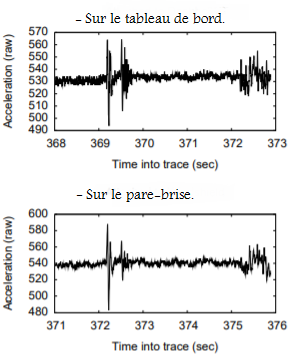
\includegraphics[width=0.75\textwidth]{Images/chapter2/positionmnt.PNG}
   \caption{Ces graphiques montrent comment le signal de l'accéléromètre (axe z) varie avec le placement à l'intérieur de la voiture selon Pothole Patrol.}
   \label{fig:smartphonePosition}
    \end{figure}


  \subsection{Méthode de récole de données}
  Pour la collecte de données, nous avons créé une application mobile qui utilise les capteurs du smartphone. Principalement l'accéléromètre et le GPS, ainsi que la vitesse de la véhicule et données d'autres capteurs tels que le capteur gyroscopique.\newline
  Tout cela sera discuté au chapitre N senction NN.

\section{Notre Approche}
Notre approche utilisera principalement le capteur d’accéléromètre comme entrées (input).
Ce Dernier signale l'accélération du véhicule le long des trois axes du capteur. \newline
 L'accélération mesurée comprend à la fois l'accélération physique du véhicule ainsi que celle de la gravité. La  mesure est signalée dans les champs Accel\_X, Accel\_Y et Accel\_Z. \newline
 En s’inspirant des travaux précédemment cités, considérer uniquement l’axe Z du capteur, en respectant le positionnement du téléphone donné, semble être une méthode à la fois simple et qui donne de bons résultats 

 Dans cette section, nous décrivons l'algorithme que nous avons développé pour détecter les conditions routières dans un enregistrement de données de capteur. \newline
Le problème de l'identification des conditions routières à partir des données de l'accéléromètre est difficile en raison de plusieurs facteurs tels que le comportement du conducteur (virages, dérapages, freinage brusque, conduite très basse, etc.) ou la grande variation et les conditions routières étranges ici en Algérie, donc notre algorithme suit 3 étapes principales:

\subsection{Windows split and Filtering}
  Cette étape est divisée en deux parties:
  \renewcommand{\labelitemi}{$\bullet$}
    \begin{itemize}
      \item \textbf{\textit{Windows split:}} Les données provenant de la partie d'enregistrement peuvent être pendant 1 mnt de conduite comme cela peut l'être pendant 1h de conduite, notre objectif principal de cette étude est de détecter l'état de la route à des distances spécifiques. L'algorithme proposé divise les données en plusieurs fenêtres en fonction de la distance et de l'heure de l'enregistrement.
      \item \textbf{\textit{Speed filtering:}} Une fois les données sont divisées en fenêtres; nous devons les filtrer avant le traitement, dans cette partie de filtrage de la vitesse (speed filtering) , les données dans lesquelles le véhicule ne se déplace pas ou se déplacent très lentement sont ignorées.
    \end{itemize}
    \textbf{ CAPTURE DE GRAPH}
\subsection{Smoothing and Threshold value}
  Une fois que l'algo a obtenu les données de filtrage, il commence à calculer la valeur moyenne de toutes les données afin d'identifier les anomalies de vibrations parmi les vibrations normales. \newline  
  Nous suivons deux méthodes pour calculer cette valeur moyenne chacune fournit un type différent de données de lissage, Nous notons que chaque méthode n'affecte pas les résultats finaux.
  
  \renewcommand{\labelitemi}{$\bullet$}
    \begin{itemize}
      \item \textbf{\textit{Average value of Waves smoothing:}} well tchika tchoka
      \item \textbf{\textit{Average value of Line smoothing:}} well tchoka tchika
    \end{itemize}
  Le moment où la valeur moyenne est détectée et en nous inspirant de nombreux articles de recherche dans ce domaine, nous avons choisi 0,8 g comme valeur sensible afin de calculer le seuil. \newline
  \textbf{AJOUTER LA FORMULE + CAPTURE DE GRAPH}


\subsection{Z-peak}
Après  que les données sont prêtes à être traitées; et que la valeur seuil est indiquée, on s'intéresse aux points de pics en dehors de cette valeur qui représentent les événements d'anomalie. \newline
Une fois cela fait, nous détectons si le niveau de la route est 0 (route lisse), 1 (route anormale) ou 2 (route très anormale) en divisant le nombre d'anomalies par la distance.
\chapter{Développement et Conception}
\label{chapter:dev}

\label{chapitre4}
		
		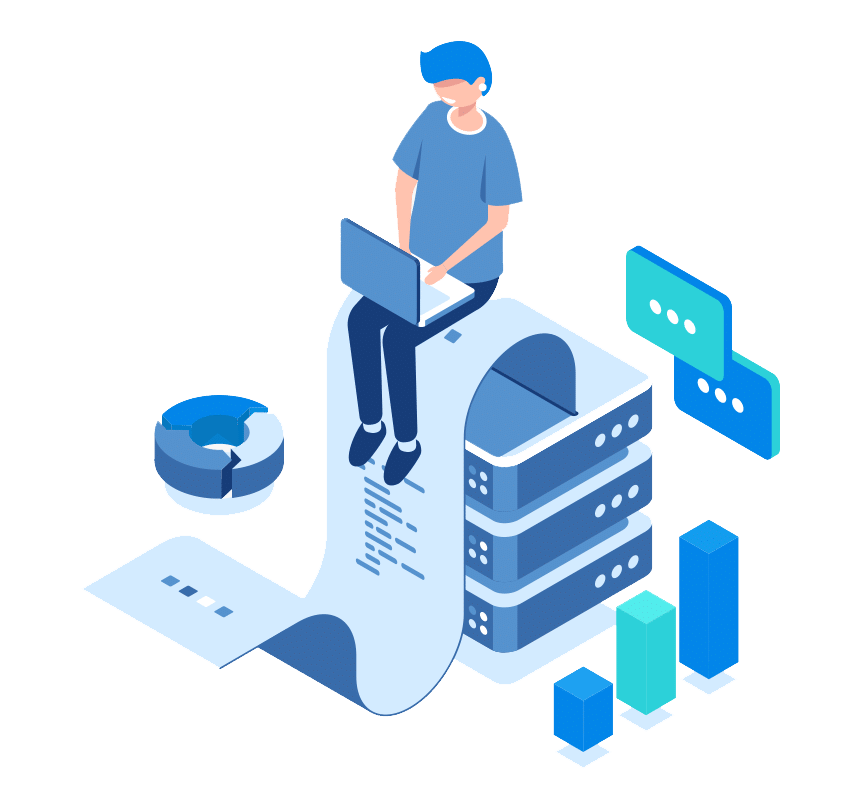
\includegraphics [width=1 \linewidth, height=0.8\textheight, keepaspectratio] {Images/chapterFigures/chFour.png}
		
	
		
		\newpage

Après avoir expliqué notre approche dans le chapitre précédent, dans ce chapitre nous expliquerons en détail comment le système proposé met en œuvre l'approche et comment elle fonctionne.

\section{Architecture du système}

Notre système se compose de plusieurs parties; une application mobile qui recueille des données, un serveur où les données en cours de traitement et stocke le résultat du traitement dans une base de données, une copie des données vers le DTP et enfin une carte interactive avec l'état de la route en temps réel pour les conducteurs (Figure \ref{fig:System}).

\subsection{Aperçu de système}
\begin{figure}[h!]
    \center
    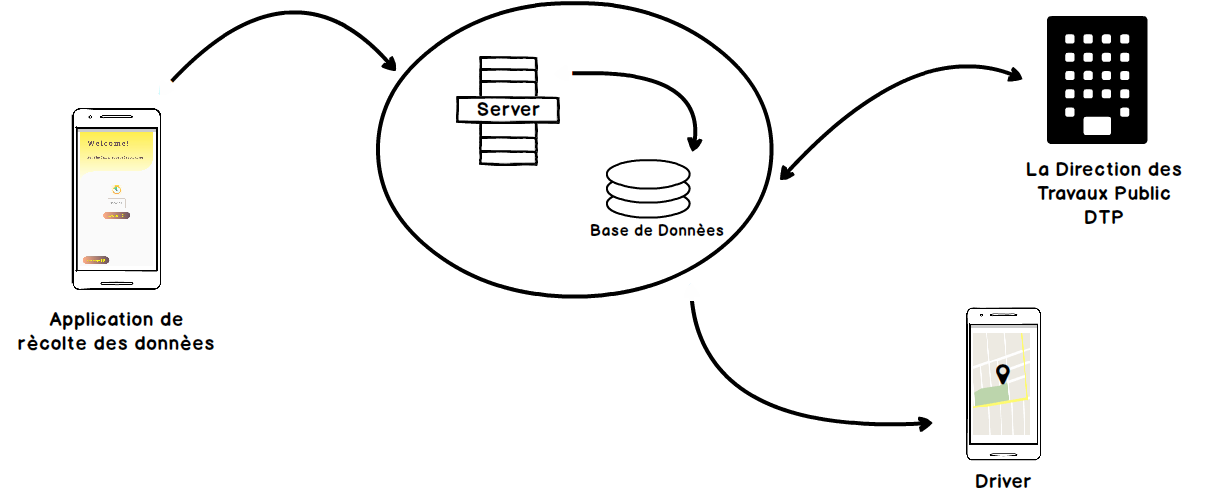
\includegraphics[width=0.75\textwidth]{Images/chapter3/systemOverview.png}
    \caption{Un aperçu du système proposé.}
    \label{fig:System}
\end{figure}

\begin{itemize}
    \item \textbf{Application de rècolte des donnèes:} Une application mobile où les capteurs du smartphone sont utilisés pour collecter les données du journal de conduite et envoyer les données au serveur.
    \item  \textbf{Server:} Après avoir reçu les données, le serveur estime l'état de la route et enregistre les résultats dans une base de données.
    \item \textbf{Base de donnèes:} Elle contient les résultats estimés de l'état de la route et l'enregistre pour être desservi par d'autres parties.
    \item  \textbf{DTP:} La Direction des Travaux Publics; la partie principale qui utilise les résultats de la base de données. Nous pouvons étendre ce système avec une application de tableau de bord pour eux, qui: \begin{itemize}
              \item Leur permettnet de surveiller régulièrement l'état de la route pour prendre plus rapidement des décisions d'entretien et de réparation.
              \item Envoyez les données fixes sur l'état de la route à la base de données après la réparation.
          \end{itemize}
    \item \textbf{Driver:} Nous pouvons également étendre ce système avec une application mobile, qui fournit au conducteur moyen une carte interactive montrant les conditions routières actuelles pour une meilleure expérience de conduite.
\end{itemize}

\subsection{Fonctionnement de système}
\begin{figure}[ht]
    \center
    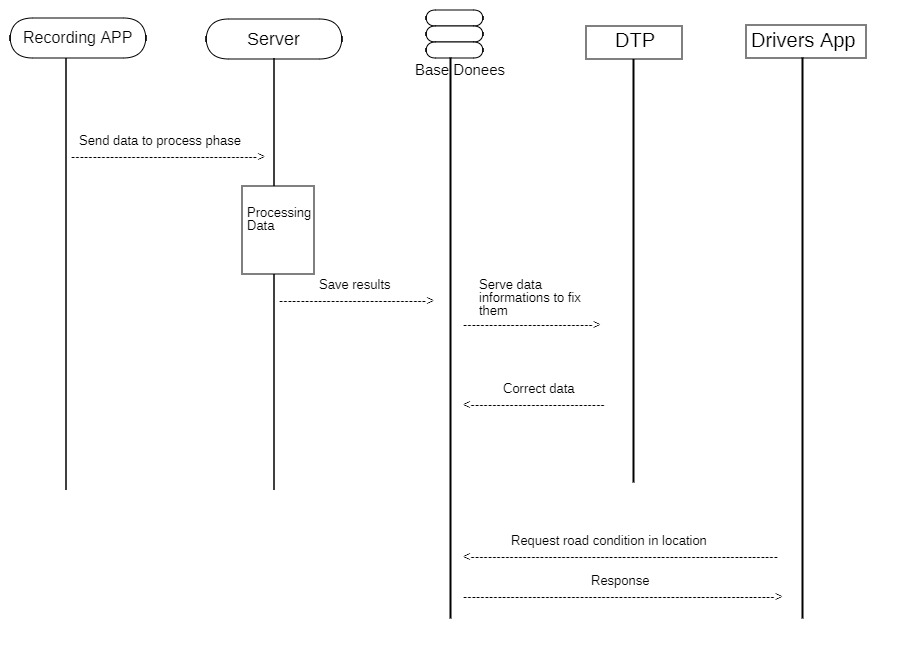
\includegraphics[width=1.2\textwidth]{Images/chapter3/diagrameSequence.jpg}
    \caption{Diagramme de séquence.}
    \label{fig:System}
\end{figure}

Notre système sous forme de diagramme montre l'envoi des données du journal de collecte de l'application d'enregistrement au serveur sous forme de fichier CSV, dès qu'il existe; Le serveur facture l'étape du processus d'enregistrement des résultats dans la base de données.

L'application de tableau de bord DTP mets à jours la base de données une fois l'anomalie corrigée, tandis que l'application Driver l'utilise pour une meilleure expérience du conducteur.



\section{Technologies utilisées}
\subsection{Python}
Python \cite{WelcomePythonOrg} est un langage de programmation qui peut être utilisé dans de nombreux contextes et est adapté à tout type d'utilisation grâce à des bibliothèques spécialisées. Il est cependant particulièrement utilisé comme langage de script pour automatiser des tâches simples mais fastidieuses. On l'utilise également comme langage de développement de prototype lorsqu'on a besoin d'une application fonctionnelle avant de l'optimiser avec un langage de plus bas niveau.

Il est particulièrement répandu dans le monde scientifique, et possède de nombreuses bibliothèques optimisées destinées aux calculs numériques \cite{PythonLangageWikipedia}.
\renewcommand{\labelitemi}{$\bullet$}

\paragraph{Pandas:}
Pandas \cite{PandasPythonData} est une bibliothèque écrite pour le langage de programmation Python permettant la manipulation et l'analyse des données. Elle propose en particulier des structures de données et des opérations de manipulation de tableaux numériques et de séries temporelles. Pandas est un logiciel libre sous licence BSD.

Les principales structures de données que propose Pandas sont les séries (pour stocker des données selon une dimension - grandeur en fonction d'un index), les DataFrames (pour stocker des données selon 2 dimensions - lignes et colonnes), les Panels (pour représenter des données selon 3 dimensions, les Panels 4D ou les Data Frames avec des index hiérarchiques aussi nommés Multi Index (pour représenter des données selon plus de 3 dimensions - hypercube) \cite{Pandas2020}.


\begin{figure}[h!]
    \center
    
\includegraphics[width=0.50\textwidth]{Images/chapter3/python_pandas.png}
    \caption{Python et Pandas Logo.}
    \label{fig:Technologies}
\end{figure}

\subsection{REST API}
API est une abréviation de:  Application Programming Interface (ou interface de programmation d’application, en français). Pour faire simple : c’est un moyen de communication entre deux logiciels, que ce soit entre différents composants d’une application ou entre deux applications différentes.

REST ou Representational State Transfer, et constitue un ensemble de normes, ou de lignes directrices architecturales qui structurent la façon de communiquer les données entre une application et le reste du monde, ou entre différents composants de la même application.

Nous utilisons l’adjectif RESTful pour décrire les API REST. Toutes les API REST sont un type d’API – mais toutes les API ne sont pas RESTful. Les API RESTful se basent sur le protocole HTTP pour transférer les informations – le même protocole sur lequel la communication web est fondée \cite{IdentifiezAvantagesAPI}.


\subsection{Flask}
Flask \cite{WelcomeFlaskFlask} est un framework open-source de développement web en Python. Son but principal est d'être léger, afin de garder la souplesse de la programmation Python.

Flask a été créé initialement par Armin Ronacher. Le souhait de Ronacher était de réaliser un framework web contenu dans un seul fichier Python mais pouvant maintenir des applications très demandées.
En 2018, Flask était élu "Framework web le plus populaire" par le Python Developers Survey. En janvier 2020, il cumulait plus de 49000 étoiles sur Github, plus que n'importe quel autre framework de développement web Python\cite{FlaskFramework2020}.
\begin{figure}[h!]
    \center
    
\includegraphics[width=0.50\textwidth]{Images/chapter3/flask.png}
    \caption{Logo Flask.}
    \label{fig:Technologies}
\end{figure}

\subsection{Flutter}
Flutter \cite{FlutterBeautifulNative} est un SDK pour applications mobiles permettant de créer des applications hautes performances et haute fidélité pour iOS et Android à partir d’une seule base de code.
L’objectif est de permettre aux développeurs de proposer des applications hautes performances qui se sentent naturelles sur différentes plates-formes.

Comme React Native\cite{ReactNativeFramework}, Flutter fournit également des vues de style réactif( se mettent à jour automatiquement lorsque les données changent ). Flutter adopte une approche différente pour éviter les problèmes de performances causé par les autres technologies hybrides, en utilisant un langage de programmation compilé "Dart" \cite{rahmouniBindex}.
\renewcommand{\labelitemi}{$\bullet$}
\begin{itemize}
    \item \textbf{\textit{Dart:}}

          Dart est un langage de programmation polyvalent développé à l’origine par Google et ensuite approuvé en tant que norme par Ecma (ECMA-408). Il est utilisé pour créer des applications Web, serveur, bureau et mobiles.
          Dart est un langage basé sur les objets (orienté objet) qui utilise une syntaxe de style C qui transcompile éventuellement en JavaScript. \cite{WhatRevolutionaryFlutter}.
\end{itemize}
\begin{figure}[h!]
    \center
    
\includegraphics[width=0.50\textwidth]{Images/chapter3/flutter.png}
    \caption{Flutter Logo.}
    \label{fig:Technologies}
\end{figure}





\section{Application de collecte}
\label{sec:app_record}
Nous avons développé une application mobile utilisant Flutter pour la collecte de données à l'aide des capteurs de téléphone. Elle peut être utilisées comme suit :

\begin{figure}[h!]
    \begin{subfigure}{.50\textwidth}
        \center
        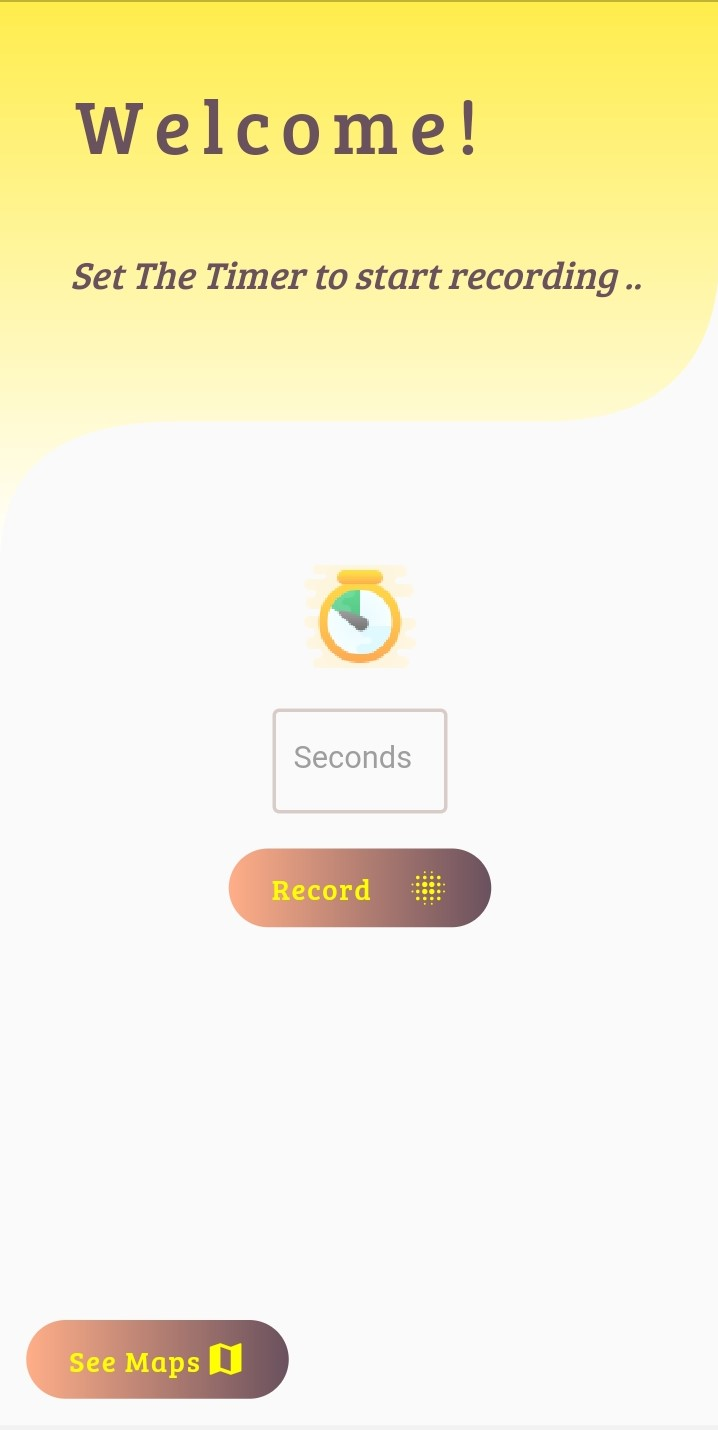
\includegraphics[width=0.50\textwidth]{Images/recordingApp/firstScreen.jpg}
        \caption{Ecran d'accueil.}
        \label{fig:Welcome Screen}
    \end{subfigure}
    \begin{subfigure}{.50\textwidth}
        \center
        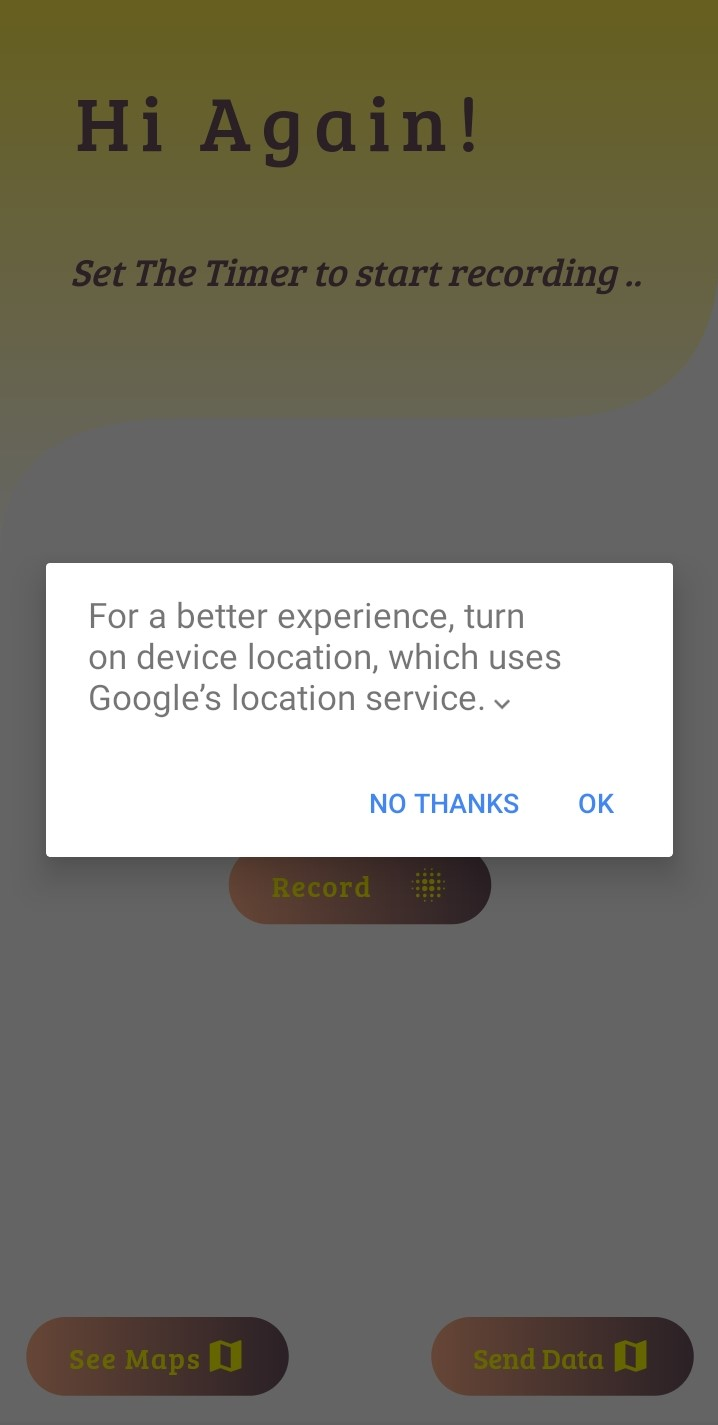
\includegraphics[width=0.50\textwidth]{Images/recordingApp/askingGps.jpg}
        \caption{Alerte d'activation GPS.}
        \label{fig:GpsAcivate}
    \end{subfigure}
    \begin{subfigure}{.50\textwidth}
        \center
        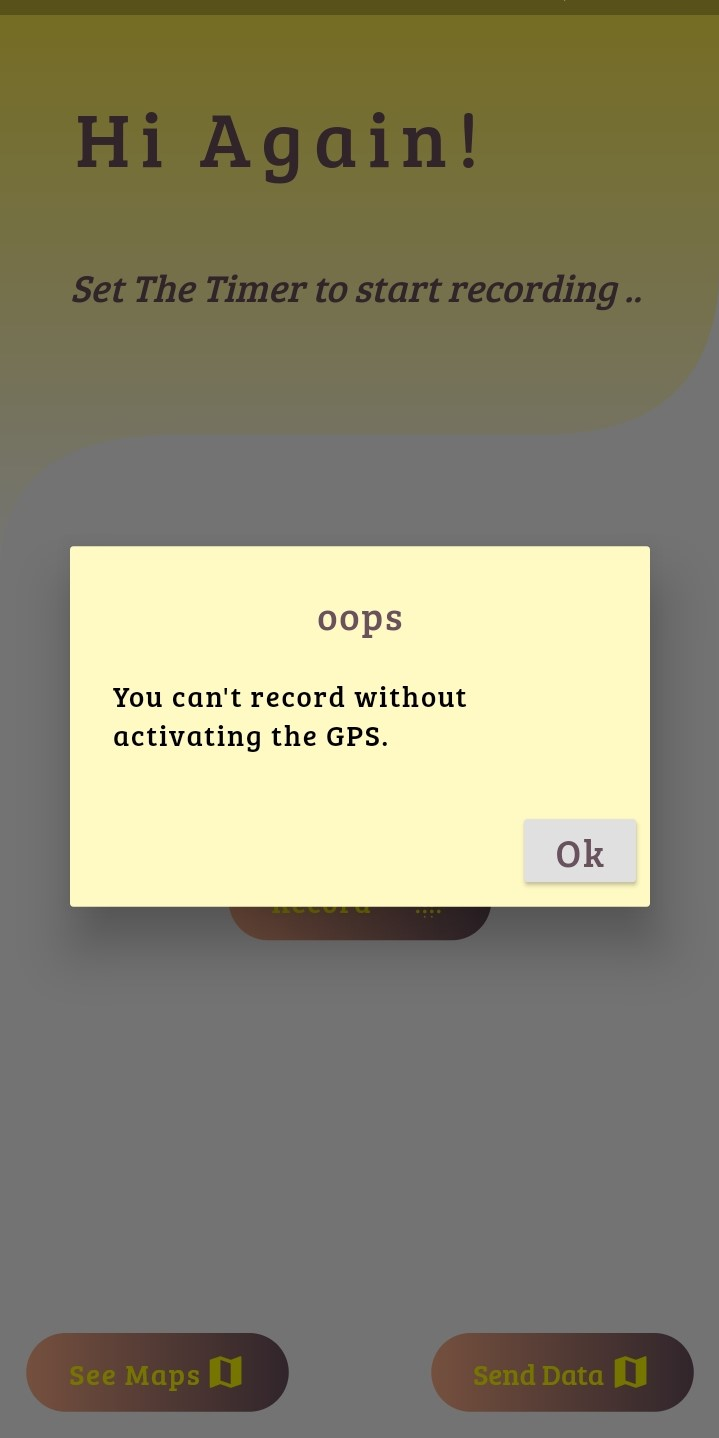
\includegraphics[width=0.50\textwidth]{Images/recordingApp/noGpsAlert.jpg}
        \caption{Notification pour activer le GPS.}
        \label{fig:gpsNotif}
    \end{subfigure}
    \begin{subfigure}{.50\textwidth}
        \center
        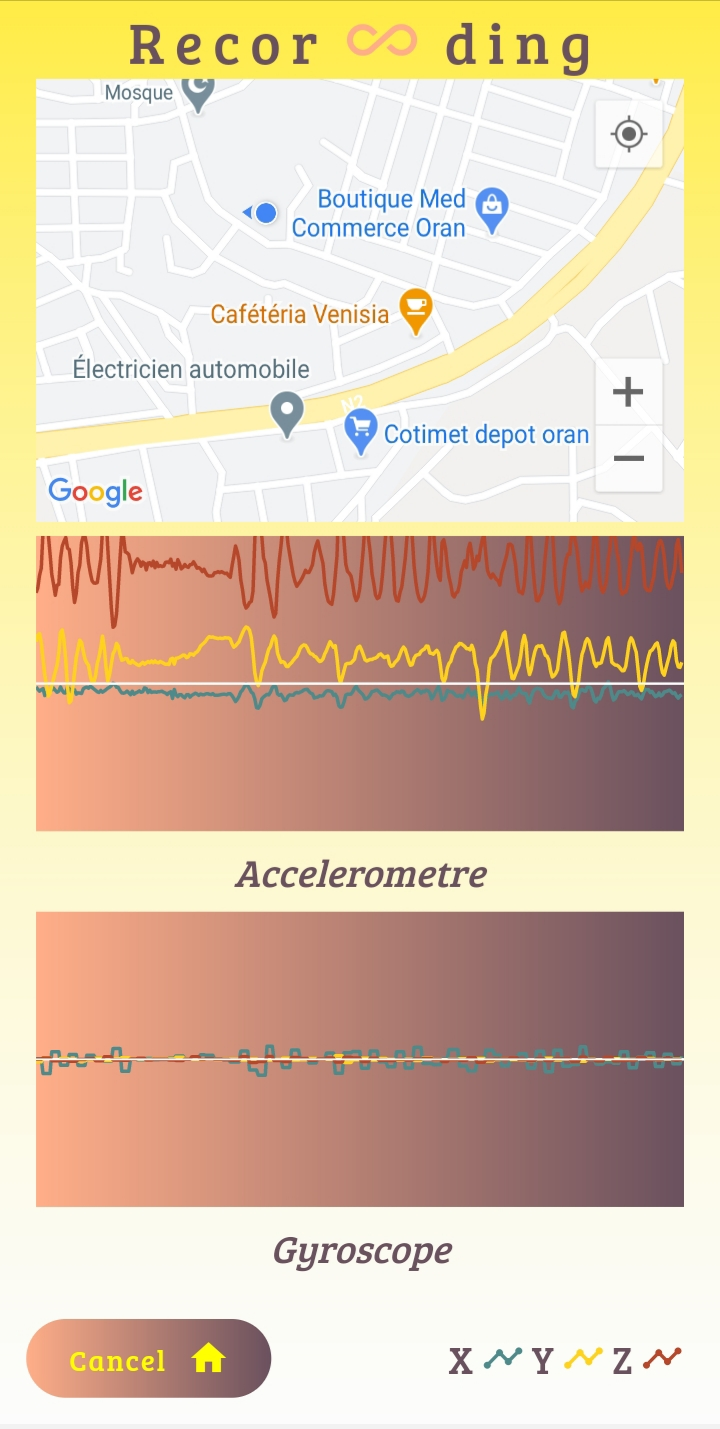
\includegraphics[width=0.50\textwidth]{Images/recordingApp/recordingScreen.jpg}
        \caption{Écran d'enregistrement.}
        \label{fig:Recording}
    \end{subfigure}
    \caption{Application de récolte.}
    \label{fig:app_recolte}
\end{figure}

\begin{itemize}
    \item D'abord, l'application demande à l'utilisateur d'entrer la durée d'enregistrement en minutes (Figure \ref{fig:Welcome Screen}).
          
    \item Deuxièmement, il lui demande d'activer le GPS (Figure \ref{fig:GpsAcivate}). Sinon, il ne démarrera pas l'enregistrement (Figure \ref{fig:gpsNotif}).
     



    \item Une fois le GPS activé et l'heure d'enregistrement entrée, l'application amène l'utilisateur à l'écran d'enregistrement, lui montrant une carte en temps réel et un graphique accéléromètre / gyroscope. Il peut annuler l'enregistrement quand il le souhaite (Figure \ref{fig:Recording}).
    
 

   

    \item Lorsque le temps est écoulé, l’utilisateur clique sur «Envoyer les données» pour que l’application envoie des données au serveur( elles seront envoyées automatiquement dans les futures versions) (Figure \ref{fig:Done}).
          \begin{figure}[h!]
              \center
              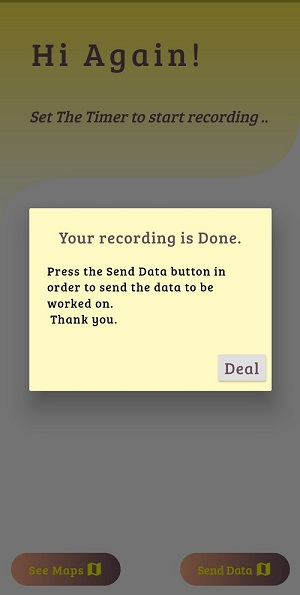
\includegraphics[width=0.50\textwidth]{Images/recordingApp/doneRecording.jpg}
              \caption{Enregistrement terminé.}
              \label{fig:Done}
          \end{figure}

          

          L'application les enregistre également sous forme de fichier CSV contenant  (Figure \ref{fig:csv}):
          \begin{itemize}
              \item La durée d'enregistrement (Time).
              \item Données de l'accéléromètre (Accel X, Accel Y, Accel Z).
              \item Données du gyroscope (Gyro X, Gyro Y, Gyro Z).
              \item Données GPS (Lat, Long).
              \item Données de la vitesse du véhicule (Speed).
          \end{itemize}
          
\begin{figure}[h!]
        \center
        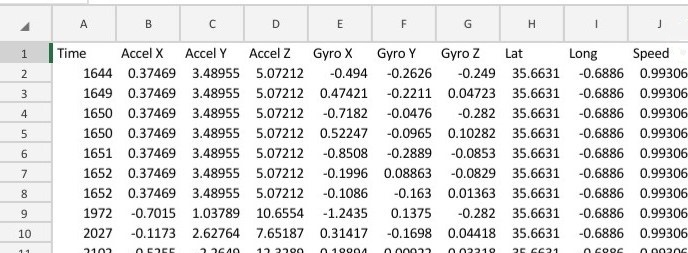
\includegraphics[width=0.95\textwidth]{Images/recordingApp/csv.jpg}
        \caption{Fichier CSV.}
        \label{fig:csv}
    \end{figure}


\end{itemize}

\newpage

\section{Serveur de traitement}
Un serveur informatique est un dispositif informatique (matériel et logiciel) qui offre des services à un ou plusieurs clients (parfois des milliers).


En fonctionnement, un serveur répond automatiquement à des requêtes provenant d'autres applications (les clients), selon le principe dit client-serveur. Le format des requêtes et des résultats est normalisé, se conforme à des protocoles réseaux et chaque service peut être exploité par tout client qui met en œuvre le protocole propre à ce service.

Dans notre implémentation, le serveur de traitement prend en charge:
\renewcommand{\labelitemi}{$\bullet$}
\begin{itemize}
    \item Le traitement des données avec l'algorithme comme indiqué dans \ref{sec:approache}, qui renvoie le Z score. 
    \item Utilise flask pour la partie de l'API, afin que toutes les autres applications concernées puissent communiquer avec le serveur, notre application principale ici est l'application Flutter \ref{sec:app_record}.
\end{itemize}
\subsection{Avantages de l'API (Application Programming Interface)}
Le server de traitement présente une API pour permettre la communication avec les autres applications. voici quelques avantages non négligeables des intégrations d'API \cite{BenefitsAPIDevelopers2019}:

\begin{figure}[h!]
    \center
    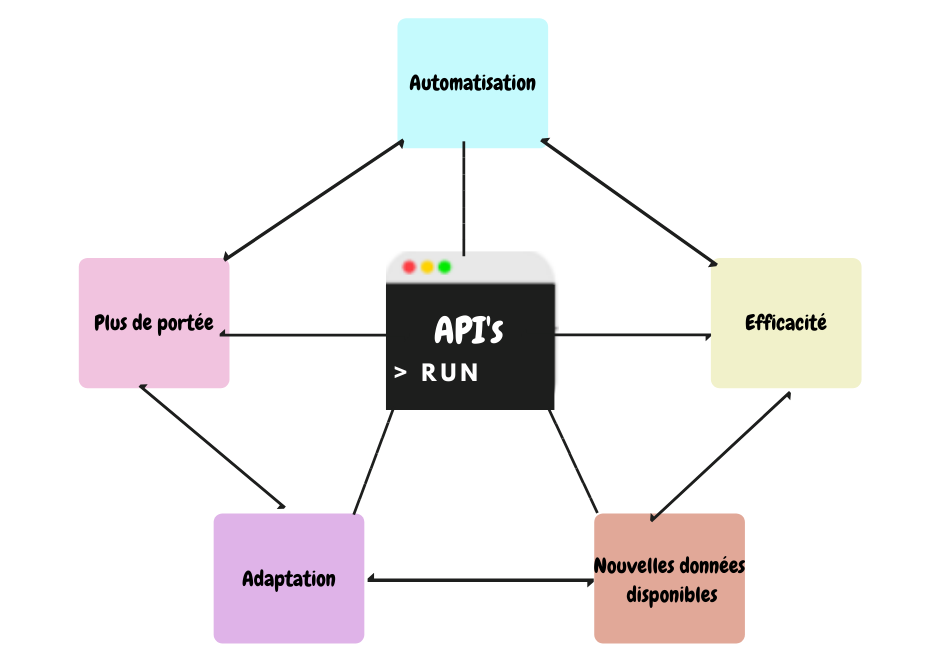
\includegraphics[width=0.75\textwidth]{Images/chapter3/apiAvantages.png}
    \caption{Avantages de l'API.}
  \end{figure}


\begin{description}
    
    \item [Plus de portée]:  En incorporant l’API dans le système, l’application peut distribuer des informations facilement à
    d’autres systèmes et peur offrir des services à de nouveaux clients (applications). La partie intéressante dans notre cas est la possibilité d'ajouter plus de fonctionnalités futures en plus du traitement de données.
     \item[Efficacité] : Une fois que vous avez accès à l'API, il est facile pour le nouveau contenu d'être publié rapidement.
     \item[Adaptation] : Chaque système doit être modifié au fil du temps, et l'API personnalisée aide à changer le système rapidement. Dans notre cas, le système (algorithme) peut être mis à jour ou complètement remplacé sans affecter les applications des clients.
     
\end{description} 

\begin{figure}[h!]
    \center
    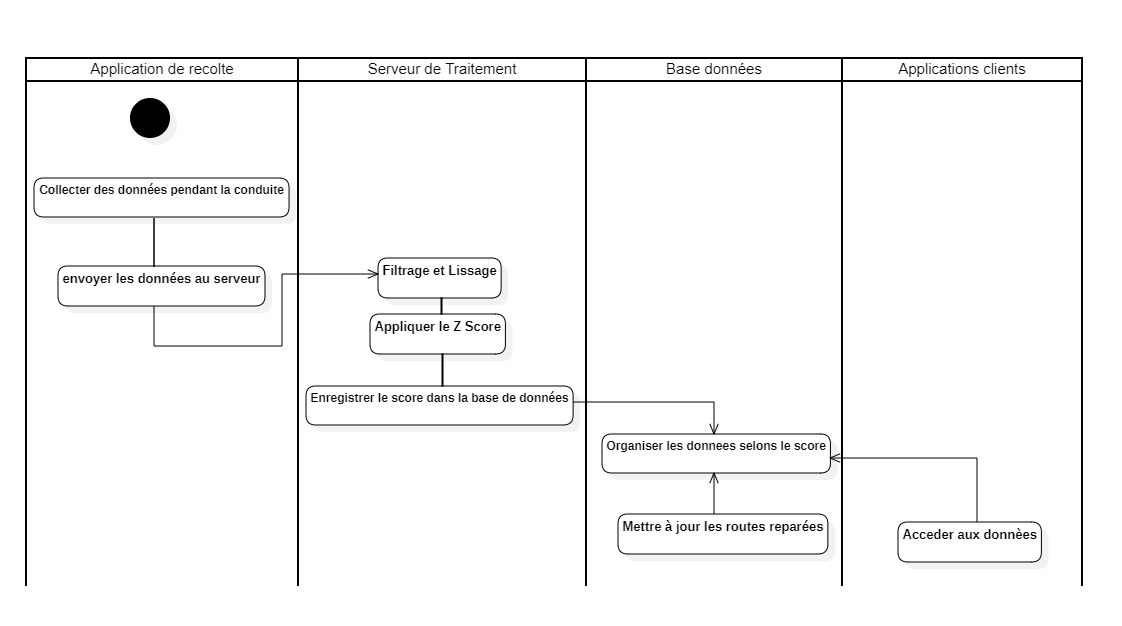
\includegraphics[width=\textwidth]{Images/chapter3/activityDiagram.png}
    \caption{Diagrame d'activités.}
    \label{activityDiagram}
  \end{figure}

  \subsection{Implémentation de l’API}
  En général, notre système suit les activités présentées dans le diagramme (\ref{activityDiagram}).
  
  
  
  Notre API travaille principalement avec deux routes:
  \begin{description}
    \item[POST /api/process\_data] : Une route qui reçoit et traite les données, puis les enregistre dans la base de données.
    \item[GET /api/road\_data] : Une route qui retourne les données stockées dans la base de données (location et score) à le application client. Elle accepte comme paramètres optionnel la position actuelle (latitude,longitude) pour retourner que les points proches de 1Km.
\end{description}

La base de données stocke le score avec un point de localisation (le centre) correspondant à la fenêtre prise, et les rend disponibles pour les différentes applications clientes.

\section{Visualisation des résultats}
Pour cette version de travail, on a essayé de visualiser les résultats obtenus depuis l’application de récolte (Figure \ref{fig:Welcome Screen}) à travers un écran Road Quality Map (Figure \ref{seeMap}) qui montre la qualité de la route de chaque 100m enregistrés à travers des cercles colorés (vert, orange, rouge), et un marqueur au centre de chaque segment avec le score correspondant. Pour plus de visibilité, les cercles verts qui représentent les segments de bonne qualité sont
cachés par défaut.

\newpage
\begin{figure}[h!]
    \center
    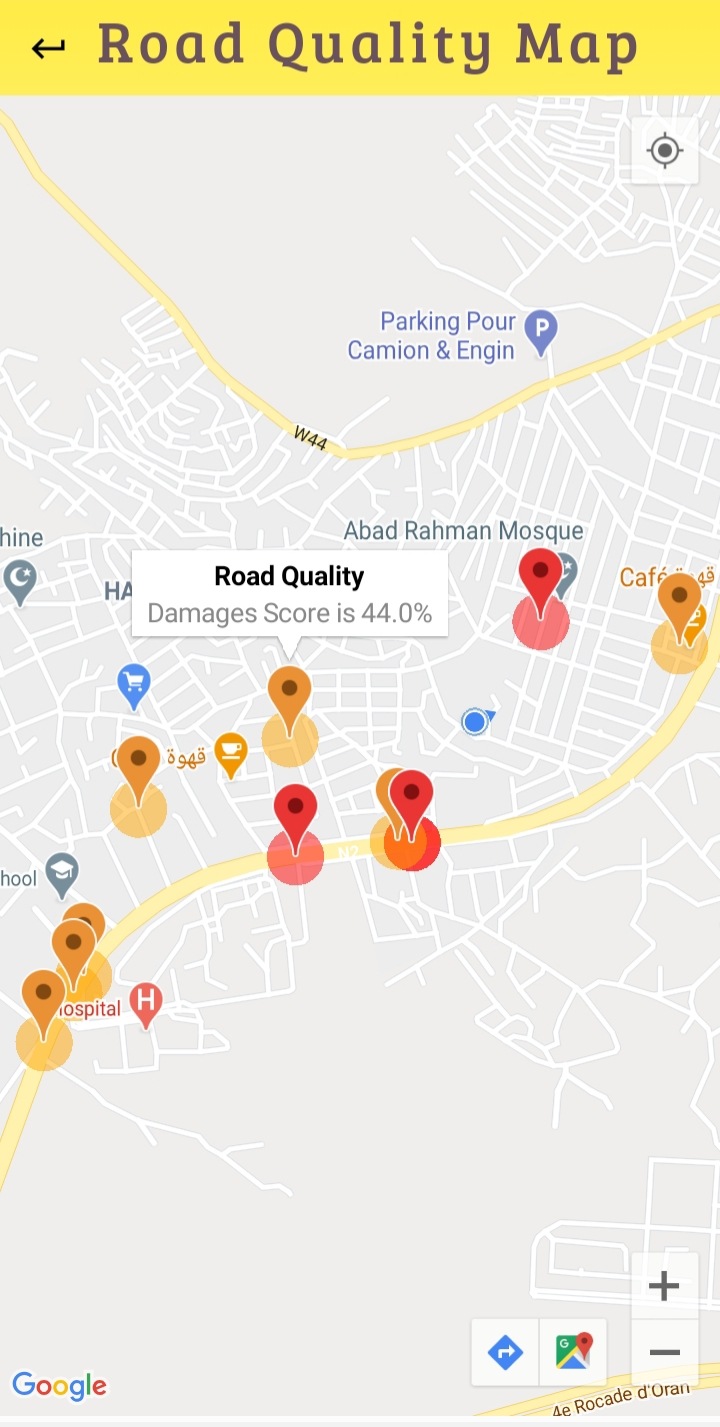
\includegraphics[width=0.50\textwidth]{Images/recordingApp/seeMap.jpg}
    \caption{Visualisation des résultats sur la carte.}
    \label{seeMap}
  \end{figure} 



\section{Conclusion}
Dans ce chapitre, nous avons décrit l'architecture de notre système, et les différentes technologies utilisées pour ce travail, nous avons également présenté comment l'application de collecte est construite et comment le serveur communique avec les différents parties. Concernant la partie base de données, elle est prévue dans les travaux futurs. Malgré les différentes contraintes (complexité du problème, manque de données claires, Pandémie actuelle), la représentation choisie pour cette première version reste suffisante et facilement extensible pour de futures améliorations.




\chapter{Conclusion et perspectives}
Le thème abordé dans ce mémoire est le traitement et analyse de données pour l'évaluation de la qualité de la route.  Nous avons commencé par montrer les différents services que nous pouvons obtenir à partir des capteurs de smartphone, et comment pouvons-nous en bénéficier dans le domaine de la détection des routes en citant plusieurs excellents travaux. Par la suite nous avons présenté l'algorithme que nous avons utilisé et comment nous l'avons lié au système qui collecte les données pour les traiter et les servir.

Ce travail reste une première version faite en utilisant les moyens relativement limités à notre disposition. Mais cela reste un bon point de départ qu’il serait intéressant à développer. Plusieurs points pourraient améliorer ce modèle, nous citons : 

\begin{itemize}
    \item Développer l'algorithme pour qu'il puisse détecter des anomalies plus spécifiques.
    \item Remplacer l'algorithme Z Score par un modèle d'apprentissage automatique.
    \item Utiliser un système plus précis pour collecter des données, comme des systèmes intégrés dans les véhicules d'état.
    \item Créer une base de données et l'associer à à l'application de la DTW pour les alerter des anomalies localisées.
    \item Faire une application pour les conducteurs, qui fournit une carte en temps réel et qui suggère la route la moins endommagée.
\end{itemize}




\bibliographystyle{abbrv}
\bibliography{bibliographie}
%\printbibliography[heading=bibintoc]
\end{document}